%%%%%%%%%%%%%%%%%%%%%%%%%%%%%
%ES100 Latex Template
%Sam Meijer '19
%Hopefully this template will serve you well.
%It is built off many other packages and templates, but I have added my own style here and there, as you should too!
%I will endeavour to explain some of the intricacies of LaTex as well as how to lay out an overall project.
%Hopefully no knowledge of LaTex is required to understand this document.
%I would highly recommend https://www.overleaf.com/learn/latex/Main_Page for further information.
%For errata, please contact smeijer11@gmail.com.
%%%%%%%%%%%%%%%%%%%%%%%%%%%%%

%Packages are included below, these are akin to libraries in other programming languages. As far as I can tell, there is no reason to reduce the number of packages included in a document. It might compile faster, but overleaf compiles fast so this should not be an issue.
\documentclass[11pt,twoside]{report} %tells the compiler that this is a 'report' style document, and the main font size.
\usepackage{setspace} %allows the use of '\doublespace' to set line spacing
\usepackage[utf8]{inputenc} %inclusion of this is optional, overleaf includes it in its compiler so it is not necessary, it may be necessary for other compilers.
\usepackage[english]{babel} %this does a few things eg allowing dates to be made by the compiler. probably best not to get rid of it
\usepackage{wrapfig} %if it is desirable to wrap text (see https://www.overleaf.com/learn/latex/Wrapping_text_around_figures).
\usepackage{graphicx} %this allows graphics to be put in easily
\usepackage{float}%this allows you to put them in good places
\usepackage[version=4]{mhchem} %this is good for chemical reactions
\usepackage{amsmath} %maths package
\usepackage{amssymb} %symbol package
\usepackage{textcomp,gensymb} %more symbols (eg \degree)
\usepackage{colortbl} %good for colouring in cells on a table
\usepackage{rotating} %allows you to rotate graphics
\usepackage{bm} %helps bold things
\usepackage{multirow} %for tables
\usepackage{longtable} %for long tables
\usepackage{pdfpages} %allows PDFs to be included in document (good if you want to include a pdf in an appendix eg)
\usepackage[nottoc,notlof,notlot]{tocbibind} %adds the bibliography to the table of contents
\usepackage{subcaption} %allows subcaption for multiple images in one graphic
\usepackage[toc,page]{appendix}
\usepackage{booktabs} %more tables
\usepackage{makecell}
\usepackage{tcolorbox}
\usepackage{sectsty}
\usepackage{titlesec}
\usepackage{multicol}

\usepackage{xcolor} %more colouring of tables

% Define primary color scheme
\definecolor{doyen-primary}{HTML}{4F46E5}
\definecolor{doyen-primary-dark}{HTML}{3730A3}
\definecolor{doyen-primary-light}{HTML}{818CF8}

% Format headings.
\titleformat{\chapter}[display]
  {\normalfont}{}{0pt}{\huge}
\sectionfont{\color{doyen-primary-dark}\bfseries}
\subsectionfont{\color{doyen-primary}}
\subsubsectionfont{\color{doyen-primary-light}}
\setcounter{secnumdepth}{0}

% Format captions
\usepackage{caption} %allows captions for graphics
\captionsetup[figure]{font=small}

% Format hyperlinks
\usepackage{hyperref}
\hypersetup{colorlinks=true}

% Set up a bibliography
\usepackage{natbib}


\usepackage[letterpaper, top=1in, bottom = 1in, right = 1in]{geometry} %this describes the layout of the document and the margins etc.
\doublespacing %self explanatory

\begin{document} % you have to do this to start the document

%%%%%%%%%%%%%%%%%%%%%%%%%%%%%%%%%%%%%%%%%%%
%For a long report such as a thesis, I would recommend thinking like programming, that is, have a short 'main' and long programs (or chapters in this case) this allows you to access each chapter easily and see the layout of the document easily.
%
%using \input{} basically puts the code specified in the argument (between the braces) into the body of the code in main
%%%%%%%%%%%%%%%%%%%%%%%%%%%%%%%%%%%%%%%%%%%

% The entire thesis is generated by the commands below, referencing the other files in this directory.

%%%%%%%%%%%%%%%%%%%%%%%%%%%%%%%%%%%%%%%%%%%
% Preamble
%%%%%%%%%%%%%%%%%%%%%%%%%%%%%%%%%%%%%%%%%%%

\pagenumbering{roman} %Roman numbering is recommended until the body
\pagebreak

\begin{titlepage}
    \def\defaultparindent{\parindent}
    \setlength{\parindent}{0cm}

    % Logo
    \begin{center}
        
\includegraphics[keepaspectratio,height=5cm]{Images/doyen-logo-new.png}\label{fig:doyen}
    \end{center}

    % Title Box
    \hrule
    \begin{tcolorbox}[colback=doyen-primary-dark]
    \color{white}
    \vspace*{1cm}
    \Large
    \textbf{Doyen: An Open Source Expert Finding Search Tool}
    \vspace{0.8cm}
    
    \normalsize

    \textbf{Muhammad Ayub$^{1}$, Jeremiah Candelaria$^{1}$, Patrick Greene$^{1}$\href{https://orcid.org/0000-0001-7052-0608}{
\includegraphics[width=0.32cm]{Images/logo-orcid.pdf}}, Edwin Lagos$^{1}$, and Nicholas Weber$^{1}$*}
    \vspace{0.8cm}
    \end{tcolorbox}
    \hrule
    \vspace{1.5cm}
    
    This project is developed in the Harvard Extension School (HES) program's CSCI E-599: Software Engineering Capstone, Spring 2023. We aim to meet the needs of our customer, Dac-Trung Nguyen, under the guidance of our instructor and co-customer, Peter Henstock.
 
    \vspace{0.8cm}
    
    $^{1}$ Division of Continuing Education (DCE), Harvard University \\
    * Correspondence: niw206@g.harvard.edu

    \begin{center}
        
\includegraphics[keepaspectratio,height=1.45cm]{Images/hes-logo.png}\label{fig:hes}
    \end{center}

    \vfill

    Degree Candidates for Masters of Software Engineering, Harvard DCE\\
    Capstone Instructor: Peter Henstock\\
    Harvard University DCE\\
    Cambridge MA\\
    \date{\today}

    \setlength{\parindent}{\defaultparindent}

\end{titlepage}

{
    \hypersetup{linkcolor=black}
    \tableofcontents
    \listoffigures 
    \listoftables
}


\vfill
\pagebreak


%%%%%%%%%%%%%%%%%%%%%%%%%%%%%%%%%%%%%%%%%%%
% Paper
%%%%%%%%%%%%%%%%%%%%%%%%%%%%%%%%%%%%%%%%%%%

\pagenumbering{arabic} %back to Arabic numbering for the rest

\spacing{1}

\chapter{Doyen: An Open Source Expert Finding Browser App}
Muhammad Ayub$^{1}$, Jeremiah Candelaria$^{1}$, Patrick Greene$^{1}$\href{https://orcid.org/0000-0001-7052-0608}{
\includegraphics[width=0.32cm]{Images/logo-orcid.pdf}}, Edwin Lagos$^{1}$, and Nicholas Weber$^{1}$*
\vspace{0.8cm}
\hrule

\section*{Abstract}
This paper presents Doyen, a web application that leverages Elasticsearch and PubMed data to identify and rank expert researchers in a given domain. Elasticsearch enables rapid search and retrieval of relevant authors based on user-specified search terms, including MeSH and general keywords. The application processes roughly 9 million of the most recent articles on PubMed, with an automated update mechanism to stay current with new research publications. The core of Doyen lies in its expert score to rank authors, considering the relevance of their work to the given search terms, publication year, and citation count, among other factors. This expert score facilitates the discovery of leading researchers within a specific domain, providing valuable insight into their research contributions. As an open-source, scalable, and user-centric application, Doyen emerges as an invaluable tool in discovering domain experts, fostering collaboration within the research community, and empowering users to make informed decisions about research partners. The user interface provides seamless search and filtering capabilities, enabling users to discover experts aligned with their unique needs. The paper also explores the project's limitations, ethical concerns of ranking experts, and potential future enhancements.  \\

{\small \textbf{Keywords:} Doyen, Elasticsearch, PubMed, Subject Matter Expertise, Expert Identification, MeSH Terms, API, Cloud } 

{
\small

\setlength{\columnsep}{30pt}
\begin{multicols}{2}

\section{Introduction}

Ascertaining the expertise of individuals within a given subject matter domain poses a significant challenge in both academic and professional contexts. Evidence-based research has become the cornerstone of almost every sector of economic growth in the industry while remaining a principal source of personal and cultural growth in the academic arts and sciences. Large organizations like governments, corporations, and academic institutions have resources to spare and established networks to draw on. They can draw experts to themselves with grants and access to other experts. However, doctors, students, professionals, and private individuals with no particular expertise may need experts far outside their networks. Health professionals might need an expert for a second opinion or a collaborator in a novel case study. A professional working in R\&D may need an expert opinion to gauge the value and viability of a new product line. Regardless of the use case, it is challenging to find individuals with subject matter experience and, even more so, determine which of them are subject matter experts. 

There are two stages to finding an expert. First, one needs to find individuals who have worked within the subject matter, and second, one must find the actual experts. Correspondingly, one might face two kinds of problems: either there are few or no experts for a subject matter because it is so narrow, or it is broad enough that there are too many experts to choose from easily. These problems are evidenced when attempting to extract experts from academic literature sources. Furthermore, these issues are present within specific domains of literature research, such as PubMed, a tool for searching biomedical and life sciences literature. 

PubMed natively offers literature search features based on specific user needs to find individuals with work published in a given subject matter. The Clinical Queries feature provides a search function with predefined filters for users to select and refine the results of relevant publications. The Single Citation Matcher tool allows citation searches based on specific user inputs and returns relevant citations of specific publications found on PubMed \cite{ref-pubmed-native}. 

PubMed articles are indexed using Medical Subject Heading (MeSH) terms. MeSH terms provide the ability to catalog biomedical publications and serve as powerful keywords used to search the PubMed database. Citation Matcher allows users to access and search within the database of MeSH terms. In addition, PubMed's Advanced Search feature allows users to build boolean queries using common terms and phrases translated into corresponding MeSH terms. However, PubMed's translation algorithm, used to convert query text into a relevant MeSH term, is imperfect, so retrieving relevant results may prove challenging if users are not well-versed in synonymically searching the 60,000 MeSH terms available \cite{ref-pubmed-updated}. Moreover, PubMed focuses on searching and retrieving literature publications rather than the experts behind the literature. While the search features are robust, PubMed's focus on literature retrieval necessitates a deeper investigation into the identification and ranking of experts. 

When faced with many authors associated with many results, ranking them as a way to narrow the ``foremost experts'' in a field can be helpful. There are numerous metrics commonly used to evaluate academic expertise. Most are simple counts, such as the number of publications or citation counts. However, awards and grant income are also widely used, and more complex metrics (often mathematical combinations of counts) are widely used. However, the limitations of numerical metrics to consistently and accurately measure expertise and ``value'' are widely acknowledged in the literature. Any single number does not tell a complete story and can often be misleading without further context \cite{ref-metrics-stack-overflow}. When metrics are combined to form comprehensive scores, they often embed subjective concepts of value that are particular to the academic landscape of the moment \cite{ref-metrics-neoliberalism}. Many metrics of value rely on the recent evaluation of the work, either directly or indirectly, so novel work that challenges current thinking may be overlooked until it becomes more widely circulated. Similarly, expert and careful work to confirm previous experiments may demonstrate a quality researcher but be overlooked because it is not flashy or new \cite{ref-metrics-games-academics-play}.

The Doyen team has created a tool that improves the issues of finding any expert in a narrow subject and finding an expert when a broad subject offers many experts. To that end, we provided a tool allowing users to search for an ``expert'' by providing adjustable post-search filters that the user deems most relevant. A government organization might value different criteria than a health professional. For example, a government organization might require that an individual be a national, while a health professional may require certain degrees and certifications. Hence, we made no intention to define what an expert should be in all contexts. We also limited searches to biomedical fields, allowing us to use the PubMed database, which contains more than 30 million publications that have been professionally indexed. Currently, we are utilizing roughly 1/3 of the most recent publications. 


\subsection{Existing Tools and Methods for Mining Publications to Find Experience}

First, we will consider what tools exist for finding experienced individuals and, in some cases, subject matter experts. Over the years, PubMed has expanded its search and filter options, yet the number of results can be overwhelming to whittle down into valuable results. To this end, developers have used PubMed's freely available API tools, such as E-Utilities and FTP, to build alternatives to searching PubMed natively. However, these tools, like PubMed, focus on searching and filtering the publications themselves rather than publication authors. One study surveyed widely used third-party PubMed tools \cite{ref-pubmed-tools}. Some tools aim to rank results or provide a better user experience, such as MiSearch and SLIM, that rank PubMed results based on user-defined weights and slider presets \cite{ref-pubmed-misearch}. Other tools seek to group results into topics or helpfully visualize outputs for users. The Anne O'Tate tool is an excellent example of both, offering users a result dashboard of relevant articles, an author list, and relevant MeSH terms associated with each. Every dashboard item displays as a link, and when clicked, a new PubMed search is performed in the background using the clicked data, giving a drill-down option into results without the user having to build multiple new searches from scratch \cite{ref-pubmed-anne-otate}. 

Several PubMed search alternatives consider options to mark and highlight search results. PubTator and PubTerm tackle this issue differently; the former offers predefined color-highlighted results based on topics, while the latter lets users make savable highlights and notes to their results as they see fit \cite{ref-pubmed-pubterm, ref-pubmed-pubtator}. Tools like LAITOR offer highly targeted queries but require software-savvy users to run MySQL queries and PHP scripts, while other tools, such as PESCADOR, abstract the need to code and make them more user-friendly \cite{ref-pubmed-pescador}.

Several alternatives combine PubMed data with outside resources to offer richer search results. For example, one tool added the ORCID database and the Elsevier API to assign author IDs to search results \cite{ref-pubmed-pmsc}. It then ranked the results by relevance and replaced the article titles with the author names, so users could easily see ranked authors based on search topics. Another tool combined the PubMed API, MeSH database, and the Orphadata directory to create author profiles dealing with rare diseases \cite{ref-pubmed-bibiometric}. Each author's profile includes their top publications on rare diseases and the top MeSH terms associated with their work. Admittedly, this tool took a naive approach to name disambiguation, combining multiple authors sharing a last name and initials. 

Other tools further combined PubMed data with outside resources by adding machine learning to filter results. One promising tool, PKG, built a knowledge graph using PubMed abstracts, NIH's ExPORTER funding information, education data from ORCID, and affiliation data from MapAffil \cite{ref-pubmed-knowledge-graph}. MapAffil is a bibliographic tool for mapping author affiliation strings to cities and their geocodes \cite{ref-pubmed-mapaffil}. The team then used a deep learning biomedical text mining model (BioBERT) to train collected data, build connections, and populate the knowledge graph. 

Like systems recommending products or entertainment, content-based filtering recommendation systems have also been used to suggest experts. Content-based filtering uses data feature vectors to make recommendations based on the user's explicit actions, such as a retail purchase or a movie watched. The model is crafted with similarity metrics and manually selected feature sets deemed suitable for the problem, requiring domain knowledge \cite{ref-google-content-filtering}. With respect to an expert finding using PubMed, the database is mined to produce features associated with authors of publications. As the user searches and finds experts, the system learns which characteristics and metrics are important to the user in evaluating expertise. 

Collaborative filtering is another machine-learning technique used to find patterns in the data. Concerning expert-finding of PubMed, this would evaluate the patterns between the user's search preferences or filters that have been previously with the experts' data and their publications to recommend a desirable match. The benefit of this type of system is that there is no need to specify the features of publications which suggest expertise. The patterns of established experts could suggest emerging experts in a field. However, the drawback is the cold start problem of initializing through explicit data before recommendations will start to become meaningful \cite{ref-google-collaborative-filtering}.

An approach to expert finding published in Applied Intelligence is a hybrid between content-based and collaborative filtering recommendation systems aiming to improve accuracy by deriving keywords from experts' Wikipedia references and using them to identify communities of experts to recommend as a set to the user. This approach uses a semantic-based method to derive expert social network relations. A k-means clustering algorithm with a proprietary homogeneity measurement was used to determine the weighted values between experts in a detected community \cite{ref-semantic-social-network}. In the PubMed Expert \& Journal Tool context, this approach would be similar to connecting experts via MeSH - Medical Subject Headings - terms and constructing a social network via similarities rather than a direct connection of terms. Although this type of approach has upsides, it, too, requires a value judgment during development regarding how to weigh similarities. 

A novel approach to using social networks to identify experts is a propagation-based approach proposed by researchers at Tsinghua University. Like PageRank, this approach makes recommendations based on their links to other experts after propagation. Unlike early PageRank, they tackled the problem where the graph nodes with the highest in-degree tend to end up in results most frequently by beginning with a local score for an expert based on the features of their work before using propagation to determine their global score. Additionally, they weight the edges of the social network graph using a proprietary algorithm to determine the propagation effectiveness \cite{ref-expert-social-network}. A significant drawback to this approach regarding PubMed Expert \& Journal Tool is that it requires its development team to assert a value judgment on the local scores and propagation coefficients. 

Despite the wide use of third-party PubMed tools, not all are convinced they enhance PubMed searches. A 2016 study comparing native PubMed to third-party search tools found that of the 76 third-party tools available, only 16 were free to access \cite{ref-pubmed-third-party}. Furthermore, those 16 offered minimal user control of parameters, filtering, and exporting compared to native PubMed. Today, many tools explored in the comparison study are either out of date or inactive. 

\subsection{Our Approach}

Ultimately, we have provided the biomedical community with an up-to-date tool that provides control of parameters and filters to find field experts. The value of our tool stands in allowing a way to search for authors in a field, as opposed to publications – which PubMed currently allows through various methods. We also leveraged the power of Elasticsearch to supply an easy-to-use yet powerful engine for finding the expertise the user requires. Elasticsearch is a distributed data search and analytics engine built for speed and scalability \cite{ref-elasticsearch}. We used Elasticsearch to index the data provided by PubMed, which we can then semantically search with keywords and MeSH terms to find publications relevant to even the most narrow specifications if they exist. Using our intermediary API, we can filter and sort these results into lists of expert authors based on user-specified criteria. We have exposed this functionality through a new user-friendly browser-based application. In addition, we aim to engage the community to receive feedback and allow others to improve and grow the project, so all our code is open-source. 

\section{Methods}

PubMed supports the mass download of their article data in over one thousand 10-30 MB compressed archives stored on an FTP server. To populate and update our index, we created a re-usable and configurable pipeline that ingests the archives, decompresses them, and enters all the individual articles into our data store. This is also a key point of data sanitation and enhancement, where we can remove faulty entries, improve the quality of existing data, and potentially augment the data with additional sorting or external sources.

It was essential that our application be able to give its response to a user's query as fast as possible, and the first part of that involves finding articles that are relevant to the expertise the user wants to find. We use Elasticsearch to build an index over the abstracts, titles, and metadata provided by PubMed. When a user performs a search in Elasticsearch, the system returns a list of documents that match their search terms, ranked by their relevance score. The relevance score is a measure of how closely each document matches the user's search terms, with higher scores indicating more relevant documents.

To calculate the relevance score, Elasticsearch takes into account several factors. One of the most important is the frequency of the search terms in the document. If a search term appears more often in a document, Elasticsearch considers that document to be more relevant to the user's search query. Another important factor is the rarity of the search terms across the entire dataset. If a search term is rare and appears in only a few documents, Elasticsearch considers those documents to be more relevant to the user's search query. Elasticsearch can also take into account the boosts that we assign to specific fields in the search query.

Overall, the relevance score is a measure of how closely each document matches the user's search terms based on a variety of factors, including the frequency of the search terms in the document, the rarity of the search terms across the entire dataset, the length of the fields in the documents, and any boosts the user has assigned to specific fields. The higher the relevance score, the more closely the document matches the user's search terms, and the more likely it is to be a relevant result.

Querying Elasticsearch directly is a skill in itself, however, and the data is still organized by articles, so we implemented a REST API to turn simple natural English keyword searches into Elasticsearch queries. The API also converts the list of articles into a list of authors, which are ranked by the relevancy of their work to the given search terms, the year their work was published, citations, and other sort options and filters. We compute a relevancy score $S_a$ for each author $a$, using the Elasticsearch scores $R_{a, p}$ for each of the papers $p$ affiliated with that author that appear in the search:
$$
S_a = \sum_{p} R_{a, p}
$$
This formulation favors authors with many highly relevant papers. More papers mean more terms, and each term weights the importance of each paper.

To make the application easy to use, we created a responsive browser application that can be accessed anywhere with internet access. The app provides the user with options for entering their terms, either as MeSH terms or as general keywords. A key advantage of Elasticsearch is that we can search for any word appearing in abstracts and titles, and we are not restricted to MeSH terms alone.

\section{Results}

\def\figwidth{0.9\textwidth}

We successfully deployed a service that provides an up-to-date search interface. We are spread across Azure, AWS, and Vercel. The service is publicly available at \url{https://doyenapp.org}.

\subsection{Our Data}

We implemented a robust, replicable deployment for our Elasticsearch instance using AWS and CloudFormation. CloudFormation encapsulates our cloud infrastructure in code so that the details that often hinder infrastructure replication are already accounted for. We were able to index 8.7 million PubMed articles from the last ten years. It takes 4.5 hours to load the content from PubMed into our Elasticsearch instance. We have set up an automatic update for the content that runs weekly. 

We deployed an API on Azure which serves our data to the user interface. Here we have implemented the ability to filter by our custom Expert Score based on the document relevancy score, the number of publications for each author, and the overall citation count. Requests to the API return hundreds of results in mere seconds. 

\subsection{User Interface}

We created a responsive browser application to facilitate ease of use, enabling access from anywhere with internet connectivity. The user interface can be divided into three sub-sections, as described below. 

\subsubsection{Search Bar and Autocomplete Drop-down Functionality}

As illustrated in \autoref{fig:ui-searchbar}, users can enter MeSH terms or general keywords and access an autocomplete drop-down list populated with over 60,000 of the most current MeSH terms sourced from PubMed. This comprehensive set of keywords allows for effortless query construction. Users can populate the search bar with multiple words while also having the option to refine the search by adding or removing keywords. 

\begin{figure*}[ht!]
    \tiny
    \centering
    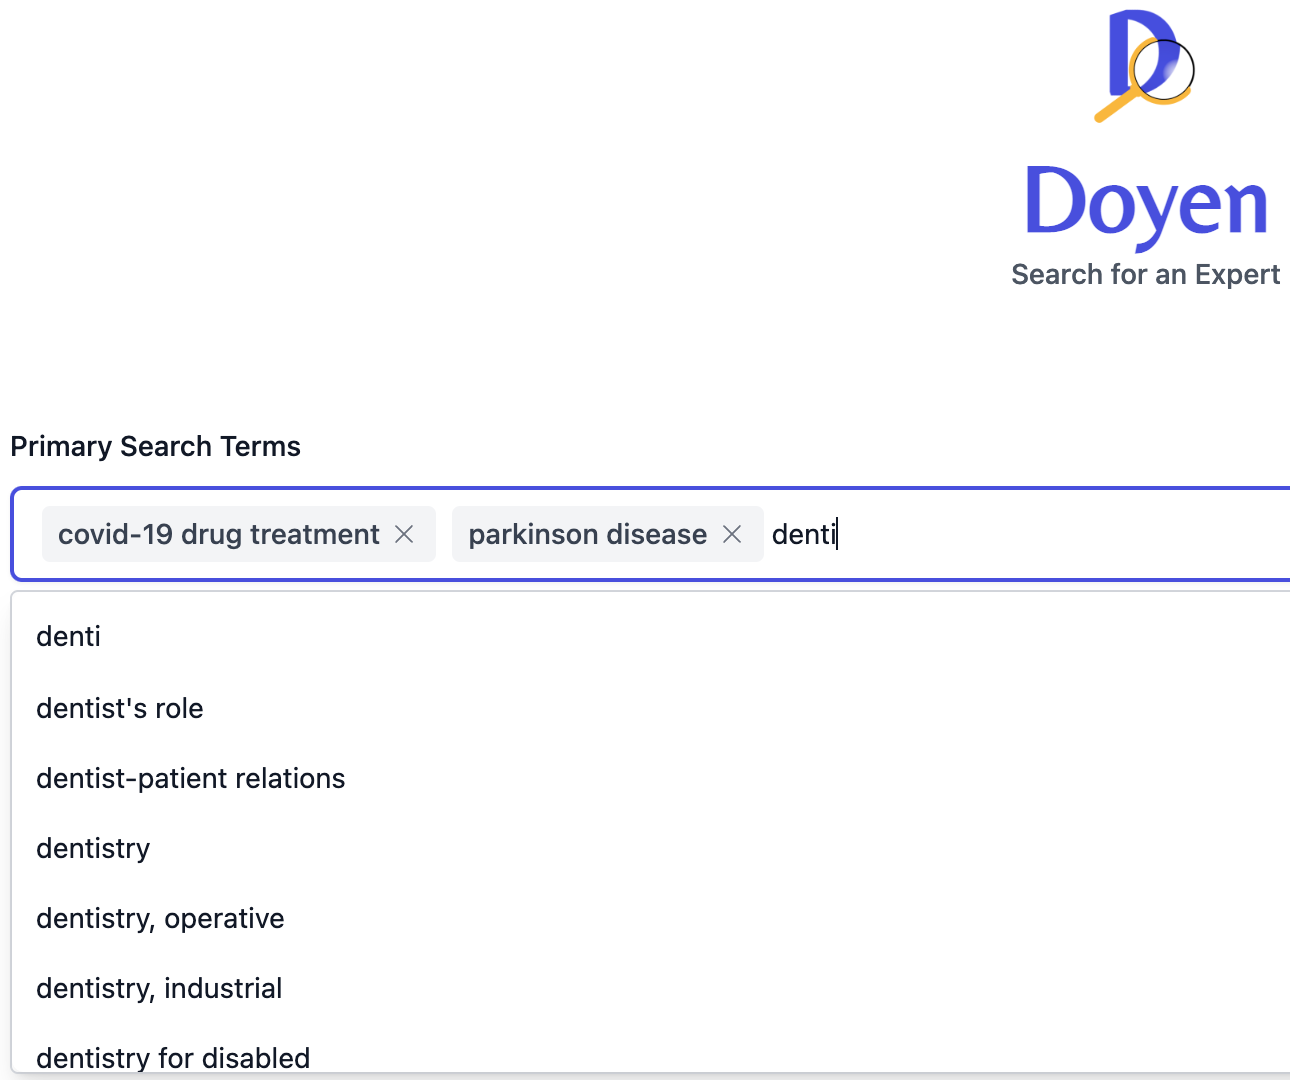
\includegraphics[width=\figwidth]{Images/ui-searchbar.png}
    \caption[Doyen App Search Bar]{\textbf{Doyen app search bar:} A view of the search bar with a user constructing a query using the autocomplete MeSH term list.}
    \label{fig:ui-searchbar}
\end{figure*}

\begin{figure*}[ht!]
    \tiny
    \centering
    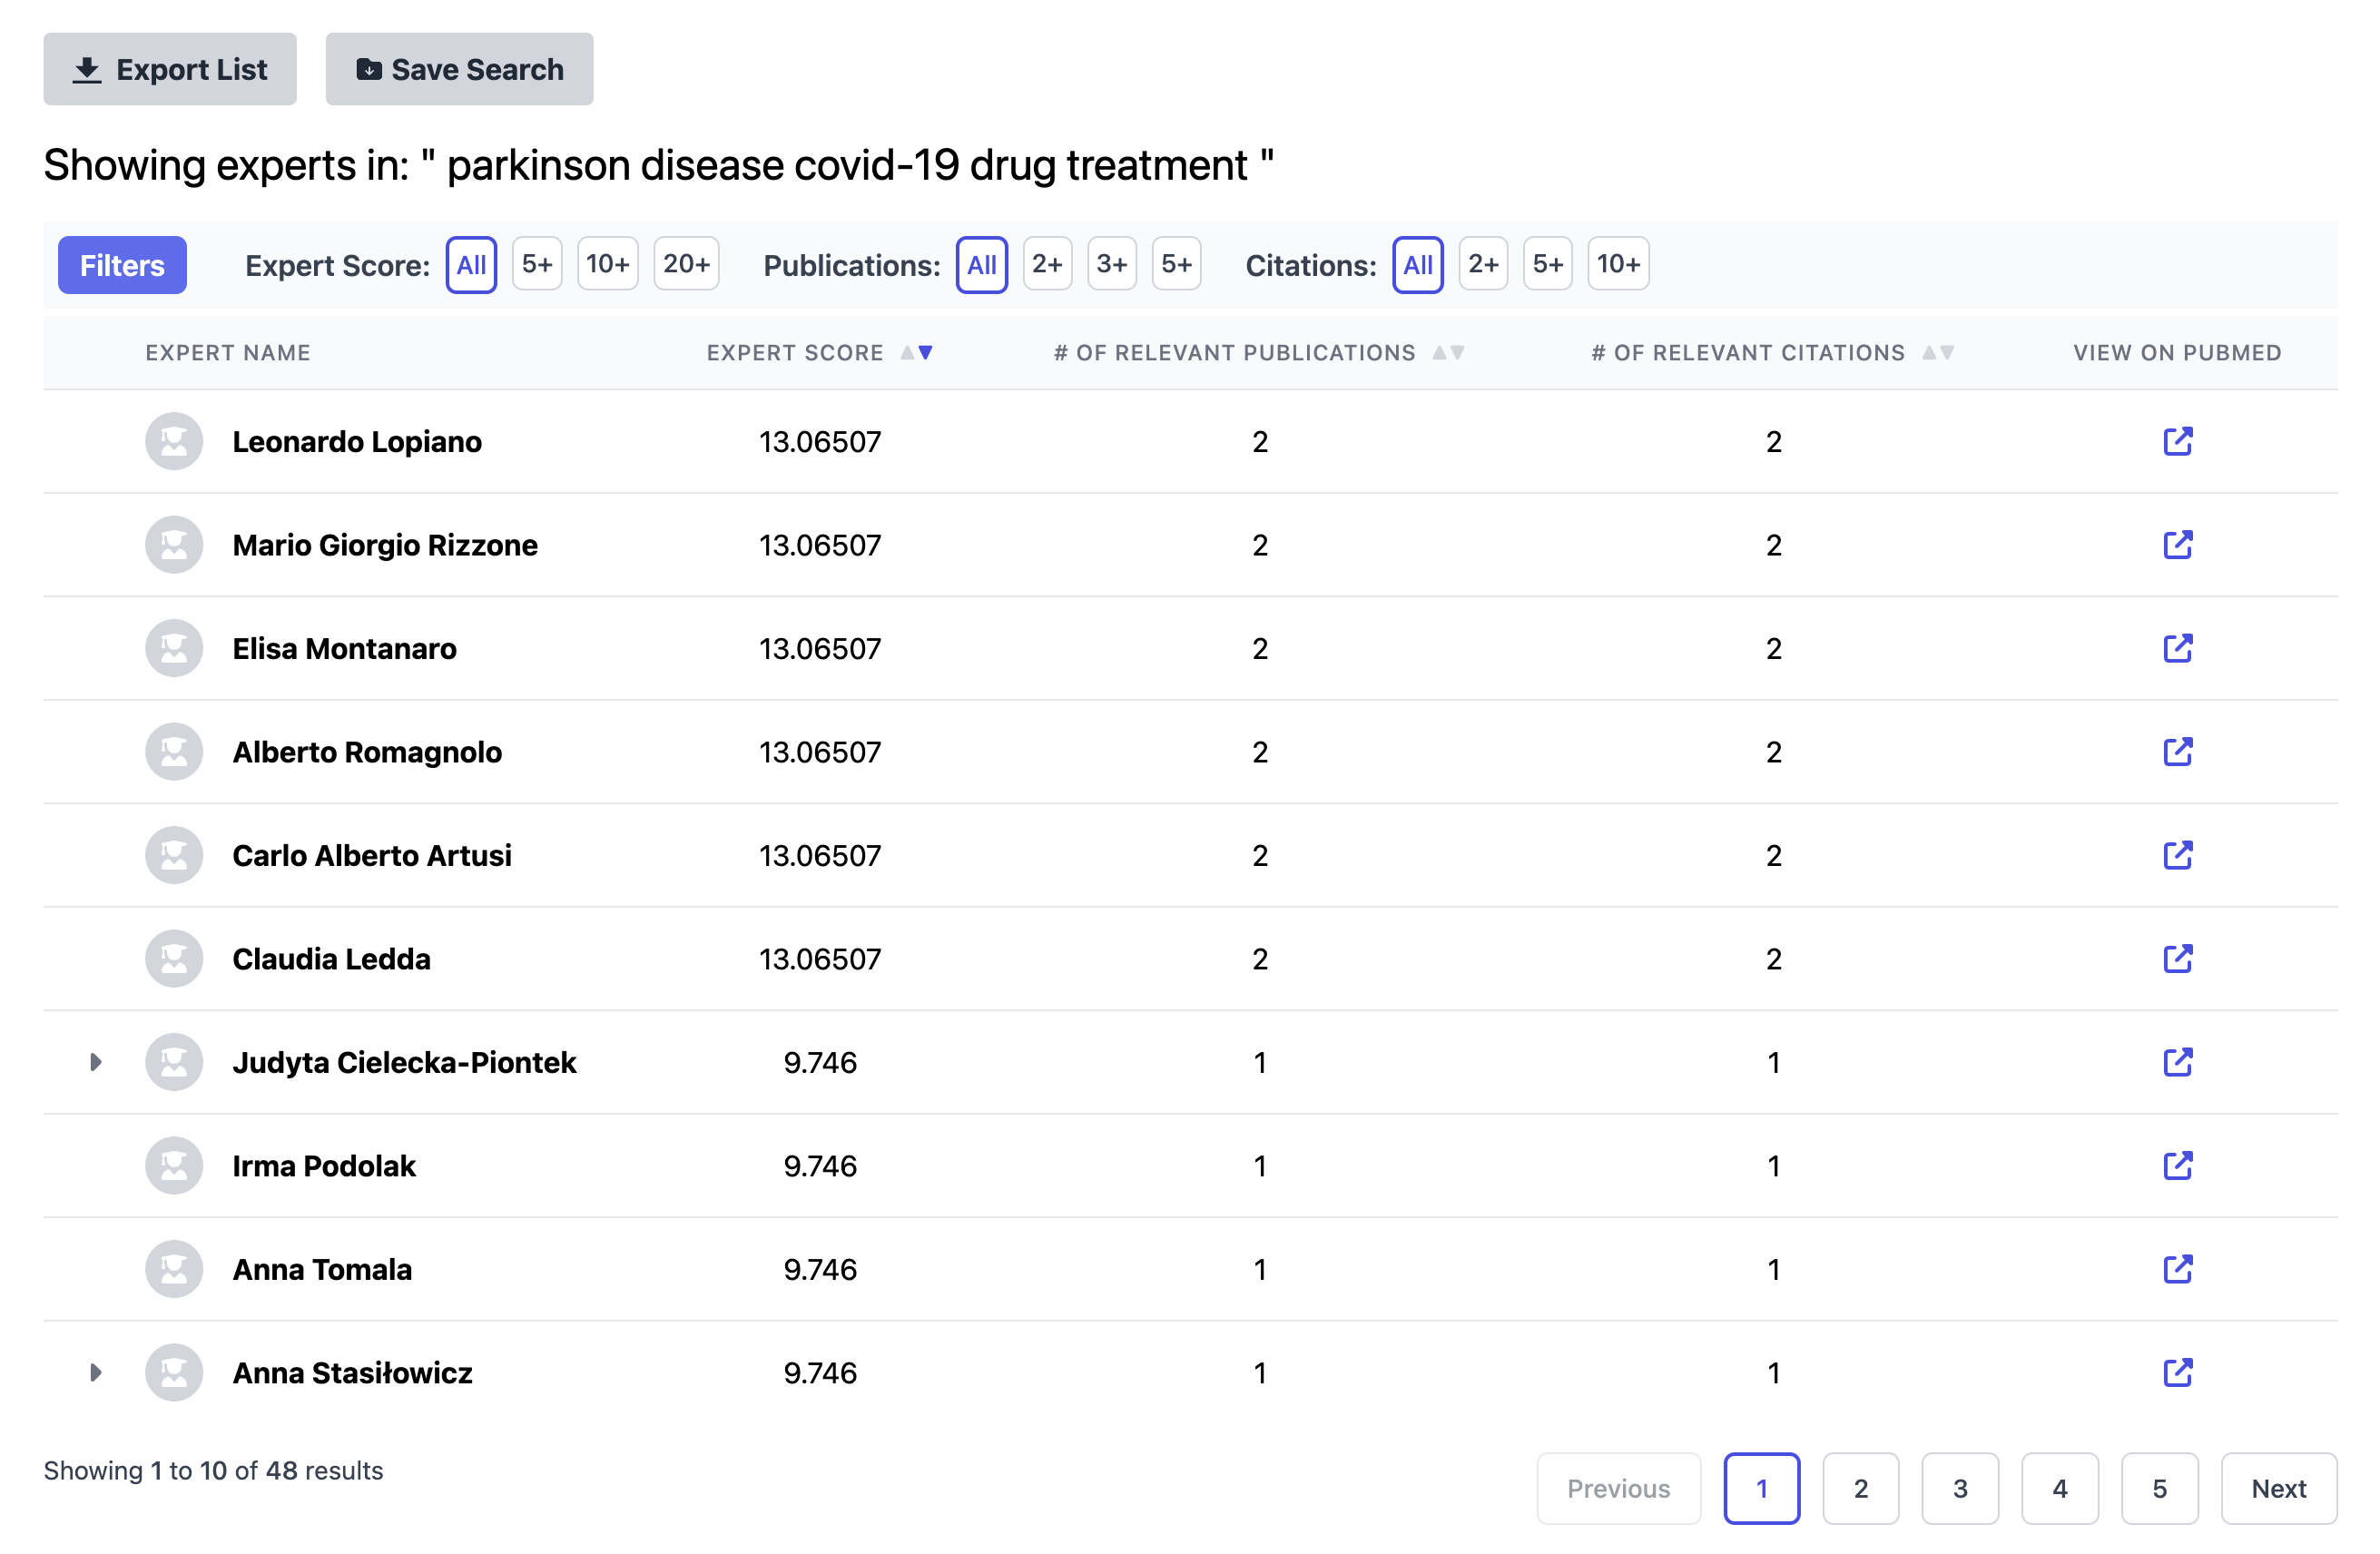
\includegraphics[width=\figwidth]{Images/ui-results.png}
    \caption[Search Results Page]{\textbf{Search results page:} A view of the results page displaying paginated expert search results, including sorting and filtering options.}
    \label{fig:ui-results}
\end{figure*}

\subsubsection{Back-End Integration and Search Results Display}

Once satisfied with their staged query, users hit ``search,'' and the search terms list is sent to Elasticsearch for a quick search of indexed PubMed publications. Elasticsearch's advantage lies in its ability to semantically search for any word in publication abstracts and titles without being restricted to MeSH terms. As shown in \autoref{fig:ui-results}, upon submitting a search query, the web application sends an API request to the back-end, which processes the query and returns a JSON object containing relevant search results. These results are then displayed on the results page, giving users an overview of the returned authors and their associated information. The interactive table presents the top 50 results sorted by the highest Relevancy Score.

\subsubsection{Filters, Sorting, and Collaborators Drop-down}

Users can sort the table based on Relevant Publication count and Relevant Citation count and filter by the number of each. The expert's section containing author identification also displays a drop-down for users to view a list of coauthors who have collaborated with the expert listed. Additionally, as shown in \autoref{fig:ui-collaborators}, users can download a PDF list of all returned authors for future reference or save their current search, allowing them to access and explore pertinent information efficiently. This functionality enhances the overall search experience provided by our web application. Users can also filter the display results by score value, publication count, and citation count and choose to view only experts with known collaborators in the drop-down list. Lastly, users can click to view relevant publications corresponding to the search directly on PubMed. 

\begin{figure*}[ht!]
    \tiny
    \centering
    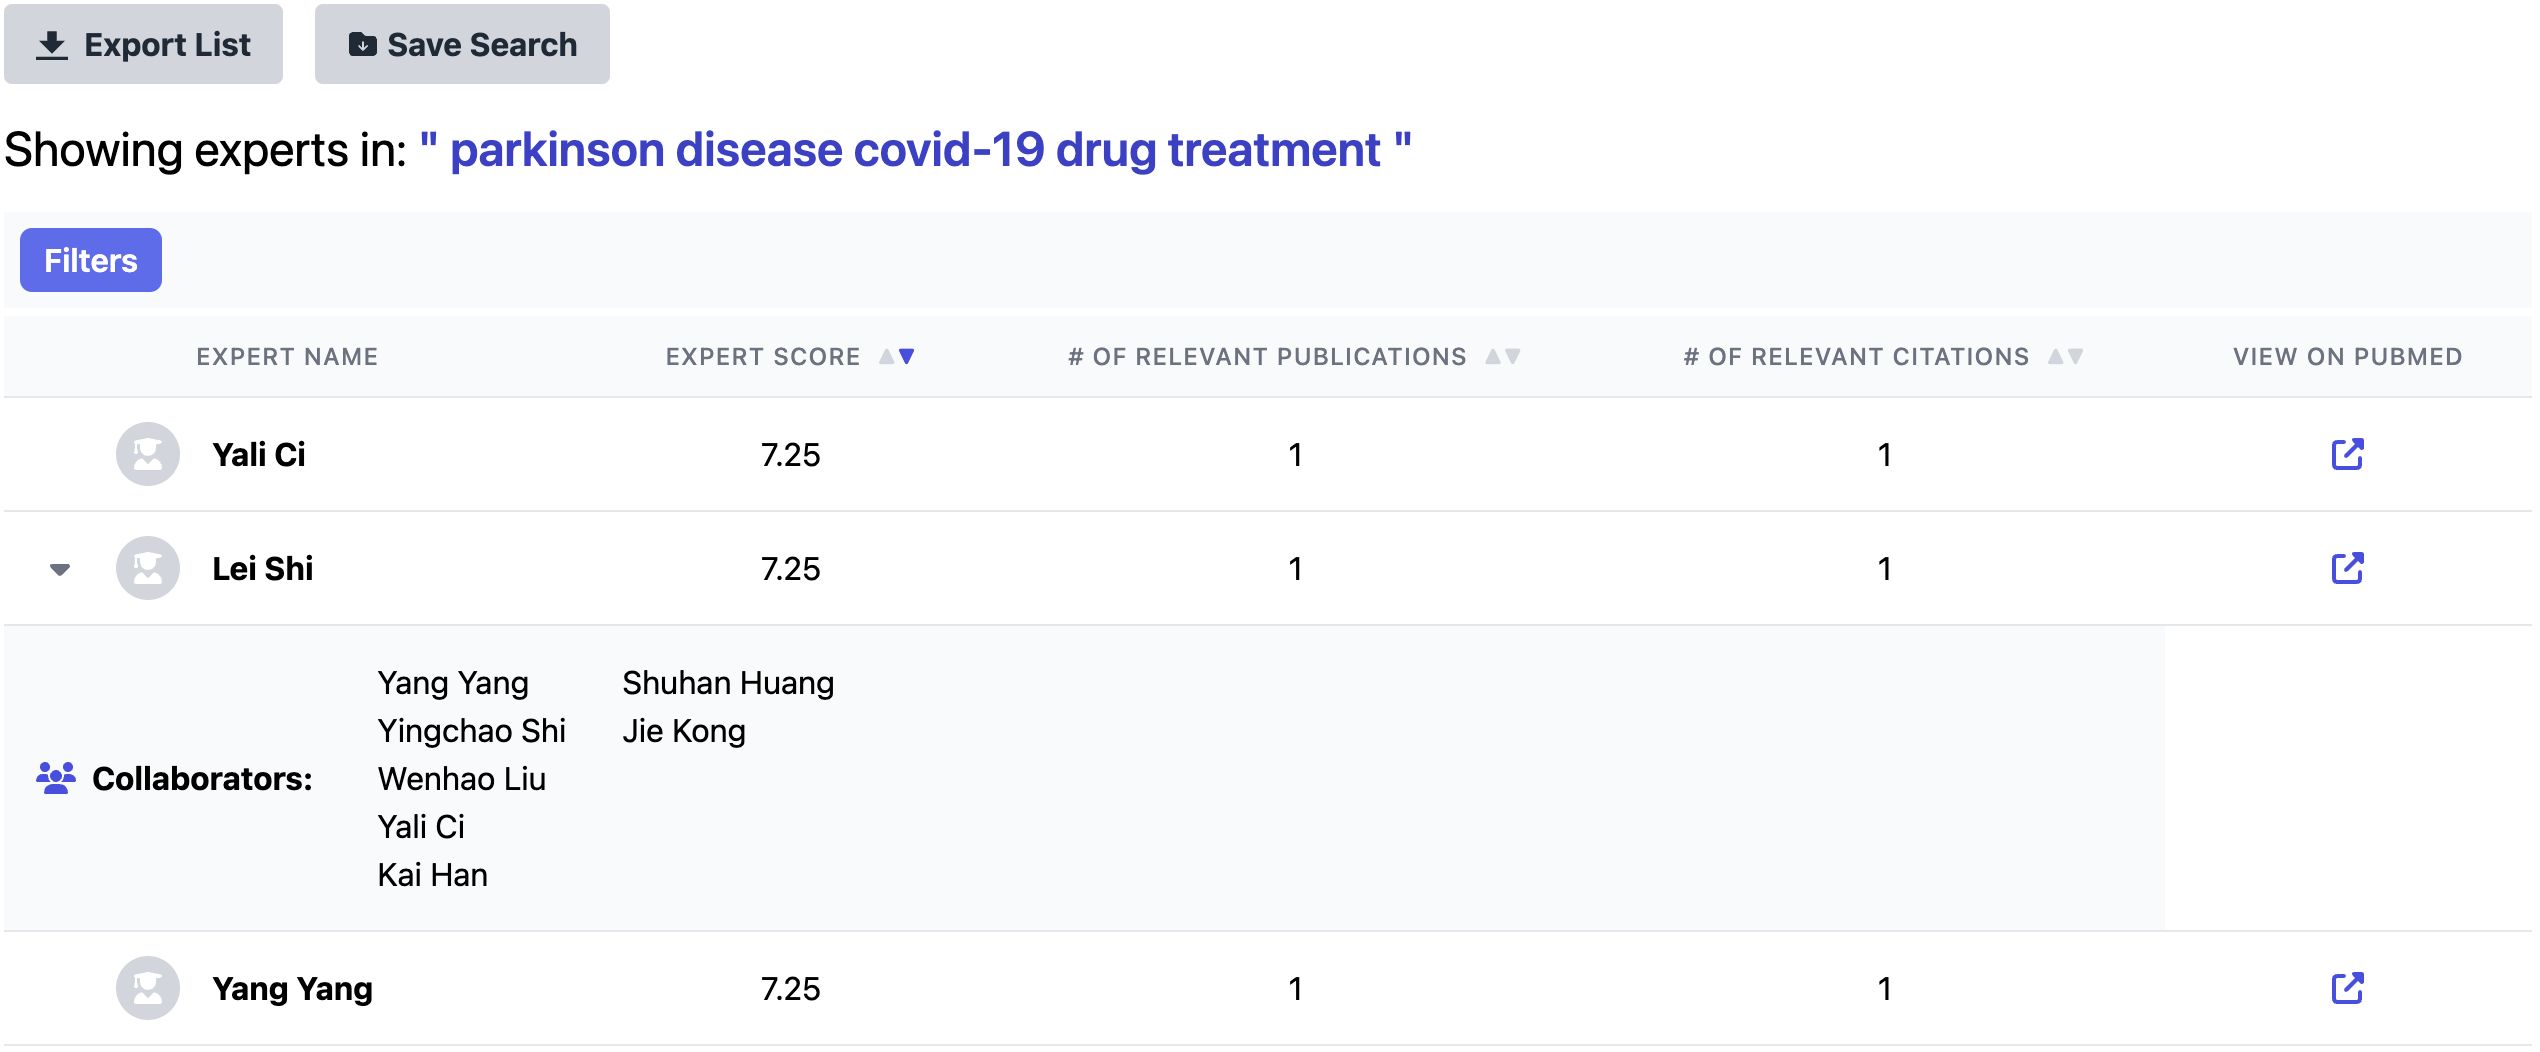
\includegraphics[width=\figwidth]{Images/ui-collaborators.png}
    \caption[Collaborators List Drop-Down]{\textbf{Collaborators list drop-down:} A view of an expert's collaborators in a displayed drop-down list.}
    \label{fig:ui-collaborators}
\end{figure*}


\section{Discussion}

We were able to create a solid foundation for this application with a valuable set of core features. However, in many ways, this is just the beginning of the app's potential.

\subsection{Limitations}

The current application does not have a way to disambiguate authors, which means that common names can dominate results. This would best be addressed using existing solutions for author name disambiguation \cite{ref-approach-author-name-disambiguation, ref-openalex}. We could also do more to map general terms into MeSH identifiers \cite{ref-approach-gilda}. However, we found that many of the queries our users wanted to make could not possibly be converted into MeSH IDs.

It is also not hard to find combinations of criteria that yield no results because there are no authors with that exact overlapping experience. We suggest the novel approach of suggesting an optimized group of individuals to meet over-constrained criteria, thus allowing us to supply a response no matter how narrow and niche the requirements are. We will use the institution data present in PubMed to let users search based on the physical locations of authors, and we will use external sources of metric data to provide other filters for author credibility and prominence.

\subsection{Ethical Considerations}

Going forward, as the application aims to grow its user base, it will be important to consider challenging ethical concerns. However, we believe that a careful examination of these ethical considerations will also suggest novel solutions that add unique value to the users of this application.

Given a large selection of individuals with experience in a subject matter, it is necessary to select a subset of that list to return to our users. A simple method to do that is to rank experts. Ranks can be as simple as counts of publications, citations, grants, or awards. A commonly used and slightly more abstract number, the h-factor or h-index, combines citation counts and the number of publications \cite{ref-metrics-methods-web}. Variants such as the m-index, which accounts for the length of the scientist's career, have also been proposed, though they appear to have minimal hold based on their absence from most of the literature \cite{ref-metrics-using-metrics}. Other numbers can be used to rank academics on their productivity and expertise, many of them domain-specific, and systems have been proposed to assemble these numerical measures into singular ranks \cite{ref-metrics-eval-biostat}, however, few seem to have caught on systemically (however grandiose the claims of the authors).

We have found in our research that the attitude towards ranking and scoring in academia has soured over the last few decades. Very little has recently been published proposing new metrics, with the most recent publications appearing in the mid-2010s. Meanwhile, metrics are frequently and increasingly used to filter out candidates for grants and jobs. This is no doubt a major cause for the shift toward critiquing the metric process in academic publications. Key among these criticisms is the way that metrics have been gamified \cite{ref-metrics-manipulation, ref-metrics-games-academics-play}, and how they create perverse incentives that reduce the quality of academic work \cite{ref-metrics-neoliberalism}, and our ability to separate experts from frauds \cite{ref-metrics-perverse-incentives}. Simply making metrics easily available and browsable can have a negative effect on relationships between academics, and the context and purpose of such metric displays must be carefully considered when creating such applications \cite{ref-metrics-resviz}.

Attempts have been made to create more comprehensive, complete, or sophisticated metrics. Some have used document metrics, including computational analysis techniques, and  considering details such as author status on a paper. The more sophisticated of these systems have become paid products, such as the Web of Science, now owned by Clarivate (previously the IP of Thomson Reuters) \cite{ref-metrics-using-metrics}. Other attempts have been made to simply establish if a person is ``expert enough'', acknowledging the lack of any single ``gold standard'', many of them using the so-called Cochran-Weiss-Shanteau (CWS) method \cite{ref-approach-to-identifying-smes}. Some of these have been aimed more at in-house employee rankings and evaluations and thus assume the ability to acquire specific input from the individuals in question. They attempted to improve on simple metrics by utilizing employee responses, then using statistical analysis to extract scores from those responses \cite{ref-metrics-cws-guide}, or use collaborator responses to create measures of ``success'', including social dispositions \cite{ref-metrics-psycho-scale}.

It is the responsibility of funding agencies and, by extension, any service that aims to serve them, to make decisions that improve the culture of practicing science \cite{ref-metrics-games-academics-play}. It is fundamentally difficult to judge the work of experts by the very nature of being experts because, by definition, an expert can do something few others can. Thus few others are qualified to judge them. Moreover, long, nuanced, qualitative descriptions of expertise are difficult to compare. This is why metrics are valuable and sought after in the first place; they are practically necessary. Metrics and rankings are fraught with limitations, creating perverse incentives that lead to the distortion of the metrics and diluting their actual value. An application that claims to identify expert individuals must balance the tension between easy evaluation, resistance to malign manipulation, and fostering adversarial behavior amongst the subjects of evaluation.

\subsection{Future Work}

In addition to addressing the key limitations, some more novel strategies are worth consideration, and the deployment and infrastructure can be improved and streamlined. For a publicly accessible and likely publicly funded project such as this, it will be essential to limit the cost of keeping the service running. To that end, the cloud utilization could be consolidated into a single provider. Future efforts would also benefit from using cheaper serverless deployments of the API and using the scalability of compute resources to use only as much computing power as is needed. Specifically, the pipeline that streams PubMed data into Elasticsearch requires significant computing power but only needs to run a few hours each week.

We could also make use of institutional information to filter by the location of the author. The primary challenge here is the poor quality of the data provided by PubMed, with some institution information blended with author emails and very infrequent institution IDs. Here again, integrating with an external source such as OpenAlex could help to resolve these ambiguities, allowing users to select experts based on proximity.

Last but not least, inspired by ethical considerations, it would be worth considering non-ranking or quasi-random strategies for suggesting experts. So long as the result meets the user's criteria, it may not be necessary to offer the best result but rather a result that is good enough. This could also unlock considerable performance improvements by reducing sort computations, which are intrinsically global, comparing each result against every other. Last but not least, this could help ensure that, should this app become widely used, the load of requests for 

\section{Conclusion}

Using PubMed and similar sources to identify experts is not new. However, there are significant challenges in using PubMed data that create technical and moral hazards. We have struck a potent blend of ideas, new and old, that together have not been seen before. We have emphasized user control to filter and select the most relevant results. We rank only as little as needed to present options that are expert enough, offering varied results when re-queried. 

We deployed a functioning application on the cloud, which is available for anyone. It has a core of valuable features and plentiful opportunities to expand. In addition, we ensure that the process can be replicated and reproduced, reducing the dependence on any few individuals and setting the stage for broader community feedback and contributions. 

\end{multicols}

\section{Software Availability}

One of the core goals of this project was to create a resource that was open-source and available for community development and feedback. All project code, including this paper, can be found in our GitHub organization (\url{https://github.com/DoyenTeam}). The code and documentation for our back-end and API can be found at (\url{https://github.com/DoyenTeam/doyen}), and our front-end can be found at (\url{https://github.com/DoyenTeam/doyenclient}). Our back-end uses Python for our ingestion pipeline and C\# for our API. The front-end is implemented using NextJS and Tailwind for styling.

The LaTex files for this paper can also be found in our GitHub organization here: \url{https://github.com/DoyenTeam/Spring2023-paper-and-report}.

\section{Data Availability}

The PubMed data is open-source, free to use, and available from their FTP server (\url{https://ftp.ncbi.nlm.nih.gov/pubmed/}). For more methods of downloading data from PubMed, see the NIH page describing downloads at \url{https://pubmed.ncbi.nlm.nih.gov/download/}.

\section{Acknowledgements}

This work was part of our capstone project for the Harvard Extension School, taught by Peter Henstock in the Spring Semester of 2023. 

\section{Author Contributions}

All authors contributed equally.

\section{Use of AI}

This section of the project made extensive use of AI tools. In particular, the following tools were used:
\begin{itemize}
    \item \href{https://copilot.github.com/}{GitHub Copilot}
    \item \href{https://chat.openai.com/}{ChatGPT}
\end{itemize}

ChatGPT was used on a free trial account, and GitHub Copilot was used on a paid account integrated with the software development tool PyCharm. ChatGPT was used extensively when formulating a CloudFormation template. We asked it to suggest chunks of the template and then asked follow-up questions to help fix it and fill in the gaps. GitHub Copilot offered suggestions for completions in the template for comments and resource definitions. The process was altogether highly integrated and iterative. We would get a suggestion from ChatGPT, apply it with some completion and input from GitHub Copilot, try to run the template, then start the cycle over again to refine it based on the results. Search engines such as Google were also used to verify the results given by ChatGPT and debug specific errors that ChatGPT and Copilot struggled to resolve. 

Our primary goal in using AI for this task was to evaluate its effectiveness and learn how to use it effectively. We found this niche to be a perfect fit for AI tools. The task was highly structured but required much manual lookup of arbitrary names and boilerplate. In addition, although finding the exact boilerplate is hard, it is easy for a human to parse its meaning. This combination of hard-to-form but easy-to-check tasks is perfect for AI. Incidentally, it is also some of the most tedious work in software development. 


%%%%%%%%%%%%%%%%%%%%%%%%%%%%%%%%%%%%%%%%%%%
% Bibliography
%%%%%%%%%%%%%%%%%%%%%%%%%%%%%%%%%%%%%%%%%%%

%\usepackage{biblatex}
%\addbibresource{references.bib}

\bibliographystyle{unsrt}

\bibliography{references}

\vfill
\pagebreak
}

%%%%%%%%%%%%%%%%%%%%%%%%%%%%%%%%%%%%%%%%%%%
% Report
%%%%%%%%%%%%%%%%%%%%%%%%%%%%%%%%%%%%%%%%%%%

\spacing{1.5}
\normalfont

\chapter{Report}

You can find our code and documentation for both local and cloud deployments on our \href{https://github.com/DoyenTeam}{GitHub organization}:
\begin{itemize}
    \item \href{https://github.com/DoyenTeam/doyen}{Doyen Back-End Code}
    \item \href{https://github.com/DoyenTeam/doyenclient}{Doyen Front End Code}
\end{itemize}
This is also where feature requests and backlog can be tracked and code additions reviewed and managed.

\section{Submission Strategy}

There are two critical barriers to publication that we will have to overcome. First, we will need to meet the standards and criteria for the journal, and second, we will have to pay for our entry into that journal. Both will be challenging to overcome, given our limited time and funds. However, we found a few journals for which our work may meet the journal's criteria and which we can consider for publication, depending on the degree of success we find before the end of the semester. We also value open-source publication, so all the journals we consider would publish our work without paywall limitations to access. 

First, we considered a journal by the Swiss publisher \href{https://www.mdpi.com/}{MDPI}: the \href{https://www.mdpi.com/journal/ijerph}{International Journal of Environmental Research and Public Health}. Based on the selection of titles listed as recent publications, this journal focuses on tools used in, as the name suggests, Environmental Research and Public Health. We have a strong case that our work would significantly benefit both communities. Publication in this journal would cost 2,500 CHF, roughly 2,755 USD. 

Second, we would consider publication with \href{https://journals.plos.org/plosone/s/journal-information}{PLOS ONE}, a journal that will accept any proper research without considering the impact. The journal is viewed by a wide readership. Although we also considered PLOS Biology, it was clear from \href{https://journals.plos.org/plosbiology/s/journal-information#loc-scope}{their scope} that our work would not meet the standards of that journal. PLOS ONE is a journal designed to publish work that does not fit neatly into the boxes of other journals, as can be seen in \href{https://journals.plos.org/plosone/s/journal-information#loc-scope}{their scope}. The fees for publishing in PLOS one could be as low as 856 USD or as high as 1,931 USD, which is still less than MDPI. This is a realistic option for the publication of our work. 

Last, we can publish in \href{https://joss.theoj.org/}{Journal of Open Source Software (JOSS)}, an open-source, peer-reviewed, free-to-publish online journal hosted using GitHub. As the name suggests, they will publish any open-source software that could impact ``the functioning of research instruments or the execution of research experiments.'' They use a modern open-science method of reviews that focuses on getting submissions up to the standards rather than weeding out submissions. If all else fails, if we can complete our work even remotely well, we should be able to publish with JOSS. 

Regardless of what journal we publish, the topic of our project has illuminated the fact that our work will be made visible to biologists through PubMed and, as these are all open-access journals, likely PMC Open Access. For example, the work published by a good friend and colleague of one of our team members -- whose experience was consulted when considering our options for publications -- was \href{https://joss.theoj.org/papers/10.21105/joss.01708}{published in JOSS}, then \href{https://pubmed.ncbi.nlm.nih.gov/32337477/}{indexed by PubMed}, and is now also \href{https://joss.theoj.org/papers/10.21105/joss.01708}{available on PMC OA}. 

\section{Development Process and Lessons Learned}

This was a large undertaking in a very short period of time. Despite initial risks, we were able to meet many of our key goals and overcame many challenges. Although we were not able to reach the fullness of our original vision, we created a real and usable application with a solid core of features.

\subsection{Risks}

There is a long history of attempts to mine PubMed for useful relationships, and there have been many specific attempts to use it to search for expertise. As such, there are many known pitfalls that may halt our project, and here we discuss those risks and our plans to try and mitigate them.

\subsubsection{Author Identity Matching}
Author identity matching is a known yet critical challenge in bibliographic databases like PubMed. Given the vast amount of publications in PubMed, it is common for multiple authors to share the same name. In such cases, it is difficult to determine which papers are written by which author, leading to inaccurate citation counts, incomplete author profiles, and decreased research visibility. This is especially true for authors with common names or those who have changed their names or institutions throughout their careers.

To combat this, we wanted to attempt to use pre-existing solutions such as OpenAlex \cite{ref-openalex}. If, for one reason or another, these did not work, we planned to fall back on using first and last names plus institutions as a unique entity. This might have over-fragmented the authors, but the effect should have been minimal in most scenarios. Furthermore, we were limiting our scope to just a few years of PubMed’s decades-long backlog, limiting the amount of institution hopping that may be present in the data.

Sadly, it turns out that we simply didn't have time to even begin to tackle this problem. As is often the case, a mountain of small and conceptually uninteresting problems took our very limited time. However, in these last few weeks, we got to the point where we encountered this problem. This problem will likely be top-of-mind for whoever takes on this project next.


\subsubsection{Off Target MeSH Terms}
While MeSH terms can be a powerful tool for finding relevant articles on a specific topic, incorrect or off-target MeSH terms can lead to inaccurate or incomplete search results. For example, a researcher may use a MeSH term like "heart attack" to search for articles on cardiac arrest, which may result in missing relevant articles that are indexed using different MeSH terms, such as "myocardial infarction" or "coronary disease."

To address the problem, we planned to use pre-existing filterings of MeSH terms. If using these still presents an issue, we would have applied some home-brew solutions.

In practice, we found a way around this problem entirely. We found that the types of query our customer were interested in searching simply could not be mapped to MeSH terms. So we allowed terms to be searched through the abstracts and titles of articles using some of the strongest features provided by ElasticSearch.

\subsubsection{Performance of Data Lookup}
At least initially, we will work with just a few years of PubMed data. We have the benefit that our results need to be up to date, and the older the actions of an author, the less relevant they are. Focusing on the recent few years should give us the most needed results. In fact, going further back may muddy our results.

In practice, our choice to use ElasticSearch seems to have largely negated this risk. We faced some limits in the kinds of queries we could make, and in particular our original goal of returning groups of authors to meet very niche requests would run into this problem, and would require new solutions.

\subsubsection{Preprocessing Compute Time and Cost}
This is somewhat in tension with the first couple of requirements, but our main measure to limit this, especially early on, is to narrow the scope of our data set as described above.

We did not end up running into this problem, largely because we kept pre-processing to a minimum. A full load only took 4 hours, which is a reasonable amount of time to be down on a Saturday night around midnight. Improvement on this point would involve some sort of rolling deployment of the latest fill from PubMed of the ElasticSearch index.


\subsection{Requirements and Progress}

We had an ambitious vision, and although we did not obtain that vision entirely, we were able to implement and deploy a useful app with a solid core of features, including some of the nice-to-haves, such as advanced filtering features.

\subsubsection{Estimating Requirements}

We have tabulated the detailed requirements for this service in \autoref{t:req-func-search-input}, \autoref{t:req-func-search-result-display}, \autoref{t:req-func-search-result-sorting}, \autoref{t:req-non-func}. Estimates are made using the T-Shirt size method, and Priorities are given using the MoSCoW method. Times are given as the milestone marker, e.g. M2 for Milestone 2.

The requirements are broken into several key aspects of the project. First, there are functional requirements that can be (more or less) concretely tested, and there are non-functional requirements that are either too soft to test, involve the methods used to meet the other requirements that are not independently testable, or are reliant on externalities that cannot in practice be tested. The functional requirements are further broken down into requirements for the search interface, the contents of the search results, and the interface for interacting with those search results.

\subsubsection{Meeting the Requirements}

We have only just begun to meet the requirements laid out in our original vision. The pace of our progress has been mixed. In particular, the lack of access to a shared cloud environment until late into the project has slowed our work considerably. However, multiple team members now have local access to our data, and we can now better utilize our team members for solving the hard problems that lie ahead.

\def\requirementwidth{11.3cm}
\def\matrixwidth{1.3cm}

\subsubsection{Search Input Requirements}

Our search interface will evolve over the course of the project, beginning with more limited options for the user and expanding as we improve our capabilities. We will allow the user to search through at least 5 years of PubMed history, with hopes to expand further as time allows. The user's input will be used to make MeSH keyword term searches on the backend, with the user directly selecting MeSH terms initially but with a parsed natural language prompt after that. In addition, we will expand to include author prominence as part of the search interface. For the detailed requirements for our search input, see \autoref{t:req-func-search-input}. 

\begin{table}[ht!]
    \tiny
    \caption{\small This table lists \textbf{functional} requirements for the Doyen service \textbf{Search Input}.\label{t:req-func-search-input}}
    \begin{tabular}{l p{\requirementwidth} c c c}
        \toprule
        \thead{ID} & \thead{Title} & \thead{Est} & \thead{Pr} & \thead{When} \\
        \midrule
        30000 & The service will search PubMed’s database for experts when requested by the user. & XL & M & M2 \\
        30010 & ... return a set of authors who have publications listed in PubMed’s database as the experts when a search is conducted for the user. & L & M & M2 \\ 
        30020 & ... conduct an expert search based on a natural language query when requested by the user. & L & M & M2 \\ 
        30030 & ... search at least the most recent 5 years of publications from the PubMed database for experts when conducting an expert search. & L & M & M3 \\
        30040 & ... return responses that accurately represent author expertise and prominence when a search is requested by the user. & M & M & M3 \\ 
        30050 & ... save a user’s search history when the user has conducted a search. & M & W & M4 \\ 
    \end{tabular}
\end{table}

\begin{table}[ht!]
    \tiny
    \caption{\small This table is the design and test traceability matrix for the \textbf{functional} requirements of the Doyen service \textbf{Search Input}.\label{t:tm-func-search-input}}
    \begin{tabular}{l p{\requirementwidth} p{\matrixwidth} p{\matrixwidth}}
        \toprule
        \thead{ID} & \thead{Design} & \thead{Tests} & \thead{Status} \\
        \midrule
        30000 & Publications from the PubMed databases are indexed into Elasticsearch for persistence and access. The Doyen API serves the UI data for the user's expert searches. & Manual, Unit, E2E & Complete \\
        30010 & The UI allows the user to execute the search. The API returns the data found in Elasticsearch. & Manual, Unit, E2E & Complete \\ 
        30020 & The UI receives a natural language query from the user to perform a search. & Manual, Unit, E2E & Complete  \\ 
        30030 & At least 5 years of publications are indexed into the system's Elasticsearch index. & Manual & Complete  \\
        30040 & Elasticsearch's relevancy scoring aids the system in searching for experts based on the titles, abstracts, and MESH terms related to their publications. & Manual, Unit & Complete  \\ 
        30050 & NA & NA & Out of Scope \\ 
    \end{tabular}
\end{table}

\subsubsection{Search Result Requirements}

Our search results will be derived, at least initially, from PubMed data. We will need to preprocess that data considerably and will query it using ElasticSearch, at least initially. The service will display the authors that were found from the query, initially as a simple list of names, but hopefully later expanding into more informative and dynamic displays. Numerous metrics will be made available, as well as the author's co-relationships and locations. Furthermore, we will allow results to show multiple authors that can meet a user constraint. We will work to make it easy for the user to evaluate the results by drilling down into authors' past publications and the metadata from those publications. Lastly, the results will be exportable by the user as a PDF. The detailed list of requirements is in \autoref{t:req-func-search-result-display}.

\begin{table}[ht!]
    \tiny
    \caption{\small This table lists \textbf{functional} requirements for the contents of Doyen service's \textbf{search results}.\label{t:req-func-search-result-display}}
    \centering
    \begin{tabular}{l p{\requirementwidth} c c c}
        \toprule
        \thead{ID} & \thead{Title} & \thead{Est} & \thead{Pr} & \thead{When} \\
        \midrule
        31000 & The service will provide expert search results based on PubMed’s database when a search is executed. & L & M & M2 \\ 
        31010 & ... display a set of authors as the results when an expert search is successful. & L & M & M2 \\ 
        31020 & ... make details of the authors available when an expert search is successful. & M & M & M2 \\ 
        31030 & ... display connections between authors and coauthors in a search result set when an expert search is successfully executed. & L & S & M3 \\ 
        31040 & ... navigate to the details of connected authors in a search result set when requested by the user. & M & S & M3 \\ 
        31050 & ... provide the total number of citations of an author’s work when an expert search is successfully executed. & M & S & M2 \\ 
        31060 & ... provide the total number of peers an author has co-authored with when an expert search is successfully executed. & M & S & M2 \\ 
        31070 & ... provide the total number of publications an author has participated in as an author or co-author when an expert search is successfully executed. & M & S & M2 \\ 
        31080 & ... provide the set of scientific journals an author has been published in when an expert search is successfully executed. & M & S & M3 \\ 
        31085 & ... provide a set of Medical Subject Headings (MeSH) associated with the expert’s publications when an expert search is successful. & M & M & M3 \\ 
        31090 & ... provide the ranking of scientific journals an author has been published in when an expert search is successfully executed. & M & S & M3 \\ 
        31100 & ... provide the author’s current institution, as determined from the PubMed database, if available, when an expert search is successfully executed. & M & S & M3 \\ 
        31110 & ... provide institutional ranking metrics associated with an author when an expert search is successfully executed. & M & S & M3 \\ 
        31120 & ... provide feedback to the user when no expert can be found for a provided expert search criteria. & S & M & M2 \\ 
        31130 & ... export the set of authors in an expert search result set as formatted text when requested by the user. & S & M & M3 \\ 
        31140 & ... save the user’s filter preferences when presenting the results of an expert search to the user. & S & C & M4 \\ 
        31150 & ... save the user’s sorting preferences when presenting the results of an expert search to the user. & S & C & M4 \\ 
        31170 & ... export the results of an expert search to PDF when requested by the user. & M & C & M4 \\
    \end{tabular}
\end{table}

\begin{table}[ht!]
    \tiny
    \caption{\small This table is the design and test traceability matrix for the \textbf{functional} requirements for the contents of Doyen service's \textbf{search results}.\label{t:tm-func-search-result-display}}
    \centering
    \begin{tabular}{l p{\requirementwidth} p{\matrixwidth} p{\matrixwidth}}
        \toprule
        \thead{ID} & {\thead{Design}} & \thead{Tests} & \thead{Status} \\
        \midrule
        31000 & The publication data is indexed into Elasticsearch and persisted. The API layer queries this data to serve the UI for the user. & Manual & Complete \\ 
        31010 & The UI displays the list of authors received from the API (via Elasticsearch). & Manual, Unit & Complete \\ 
        31020 & The UI displays author metric details as a table after a search retrieves a set of experts based on aggregate queries performed at the API level.  & Manual, Unit & Complete \\ 
        31030 & The UI displays all co-authors the expert has published with. When the expert has a set of collaborators who have authored works with them, this list is presented as an accordion in the UI as part of the details table. & Manual, Unit & Complete \\ 
        31040 & The co-author links displayed in the UI will bring the user to said co-author's details page. & Manual & Partial \\ 
        31050 & The UI provides a citation count related to the search based on aggregate queries performed at the API level. & Manual & Complete \\ 
        31060 & The API provides a list of co-authors related to the search. When these authors have a known PubMed Identifier, the UI can find the details of this user. & Manual & Partial \\ 
        31070 & The UI provides a publication count related to the search based on aggregate queries performed at the API level. & Manual & Complete \\ 
        31080 & The API provides a publication set related to an expert's ID. This is not yet present in the UI. & Manual & Partial \\ 
        31085 & NA & NA & Incomplete \\ 
        31090 & NA & NA & Incomplete  \\ 
        31100 & NA & NA & Incomplete \\ 
        31110 & NA & NA & Incomplete \\ 
        31120 & The UI shows the set or empty set of experts for the search. If the set is empty, the text is displayed to the user, informing them of this. & Manual & Complete \\ 
        31130 & The UI allows the user to export the search results as a PDF. & Manual & Complete \\ 
        31140 & NA & NA & Out of Scope \\ 
        31150 & NA & NA & Out of Scope \\ 
        31170 & The UI allows the user to export the search results as a PDF. & Manual & Complete \\
    \end{tabular}
\end{table}

\subsubsection{Search Result Sorting and Filtering}

Once the search results are reported, the service will give the users multiple tools for drilling down into the results by allowing them to sort by various rankings and other metrics, time range of publication matches, and geographical location as determined by their institution. The detailed list of requirements can be found in \autoref{t:req-func-search-result-sorting}.

\begin{table}[ht!]
    \tiny
    \caption{\small This table lists \textbf{functional} requirements for the Doyen service's \textbf{search result sorting and filtering}.\label{t:req-func-search-result-sorting}}

    \centering
    \begin{tabular}{l p{\requirementwidth} c c c}
        \toprule
        \thead{ID} & \thead{Title} & \thead{Est} & \thead{Pr} & \thead{When} \\
        \midrule

        32010 & The service will sort the set of expert search results by the number of times an author’s work has been cited when requested by the user. & M & S & M3 \\ 
        32020 & ... sort the set of expert search results by the average rankings of scientific journal publications of each author when requested by the user. & M & S & M3 \\ 
        32030 & ... sort the set of expert search results by the total number of publications of each author when requested by the user. & M & S & M3 \\ 
        32040 & ... sort the set of expert search results by rankings of their current institution of each author when requested by the user. & M & S & M3 \\ 
        32050 & ... sort the set of expert search results for an author by metrics of their co-authors when requested by the user. & M & S & M3 \\ 
        32060 & ... sort the set of expert search results by the total citation count of each author when requested by the user. & M & S & M3 \\ 
        32080 & ... sort a set of experts by geographical distance measured between the user and the expert’s institution when requested by the user. & L & W & M4 \\ 
        32070 & ... filter the set of authors in the search results by a time range when the user specifies a start and end date. & S & S & M2 \\ 
    \end{tabular}
\end{table}

\begin{table}[ht!]
    \tiny
    \caption{\small This table is the design and test traceability matrix for the \textbf{functional} requirements for the Doyen service's \textbf{search result sorting and filtering}.\label{t:tm-func-search-result-sorting}}

    \centering
    \begin{tabular}{l p{\requirementwidth} p{\matrixwidth} p{\matrixwidth}}
        \toprule
        \thead{ID} & \thead{Design} & \thead{Tests} & \thead{Status}  \\
        \midrule

        32010 & The UI can set the sorting and filtering preferences of the user in its request to the API. & Manual, Unit & Complete \\ 
        32020 & NA & NA & Incomplete \\ 
        32030 & The total number of publications to journals is a sortable attribute of a search's results from the UI. The author's current institution ranking is a sortable attribute of a search's results from the UI. & Manual, Unit & Complete \\ 
        32040 & NA & NA & Incomplete \\ 
        32050 & An author's set of co-authors to published journals is available from the API, but not yet integrated with the UI. & Manual & Partial \\ 
        32060 & The number of citations for an author's work is a sortable attribute of a search's results from the UI. & Manual, Unit & Complete \\ 
        32080 & NA & NA & Out of Scope \\ 
        32070 & The user can search within the time range using the UI, which will send the time range parameters when communicating with the API. & Manual, Unit & Complete \\ 
    \end{tabular}
\end{table}

\subsubsection{Non-Functional Requirements}

There are many things that will make a service good and valuable that are not easy to test. Things like its reliability and availability, its ability to scale smoothly with changes in demand, its accessibility to various devices, its performance, and ultimately how useful the users find its results. Although not testable, these requirements are no less essential to defining the scope and challenges of our project.

As stated above, we aim to deploy a state-of-the-art service with modern standards of reliability and availability, including ensuring the website is mobile-friendly. Although the expected maximum load on the service is not expected to be high, we will ensure that those modest requirements are thoroughly met and that users get prompt responses that they find generally correct and satisfying. The full list of requirements can be found in \autoref{t:req-non-func}.

\begin{table}[ht!]
    \tiny
    \caption{\small This table lists the \textbf{non-functional} requirements for the Doyen service.\label{t:req-non-func}}
    \centering
    \begin{tabular}{l p{\requirementwidth} c c c}
        \toprule
        \thead{ID} & \thead{Title} & \thead{Est} & \thead{Pr} & \thead{When} \\
        \midrule
        40000 & The service will be publicly available when requested by the user. & S & M & M2 \\ 
        40010 & ... be available 95\% of the time when requested by the user. & L & M & M2 \\ 
        41000 & ... be able to process at least 1000 expert search queries per day when requested by users. & M & M & M3 \\ 
        42000 & ... be accessible by a web browser when the user accesses it. & S & M & M2 \\ 
        42010 & ... provide mobile-friendly views when the user accesses it. & L & S & M3 \\ 
        43000 & ... provide expert search results in under 10 seconds 95\% of the time when requested by the user. & M & M & M3 \\ 
        44000 & ... be intuitive to use for expert search by at least 80\% of users when they search for an expert. & M & S & M2 \\ 
    \end{tabular}
\end{table}

\begin{table}[ht!]
    \tiny
    \caption{\small This table is the design and test traceability matrix for the \textbf{non-functional} requirements for the Doyen service.\label{t:tm-non-func}}
    \centering
    \begin{tabular}{l p{\requirementwidth} p{\matrixwidth} p{\matrixwidth}}
        \toprule
        \thead{ID} & \thead{Design} & \thead{Tests} & \thead{Status}\\
        \midrule
        40000 & The system is publically available: https://doyenapp.org/ & Manual & Complete \\ 
        40010 & All system components are hosted by cloud provider platform-as-a-service resources. These each has general availability of more than 99 percent. Despite that, the system would be unavailable if any cloud resource failed (approximately 1 percent chance for each), and the union of all system component availabilities still exceeds 95 percent. & Analysis & Complete \\ 
        41000 & All system components are hosted on scalable cloud architectures, which can handle this load entirely through scaling vertically. & Manual, Analysis & Complete \\ 
        42000 & The system is publically available: https://doyenapp.org/ & Manual &  Complete \\ 
        42010 & The front-end is designed and implemented in React with mobile-first responsiveness patterns. & Manual, Analysis & Complete \\ 
        43000 & The system is hosted on public cloud infrastructure using HTTP communication. Elasticsearch indexes the data for access to the user via the UI and API. & Manual, Analysis & Complete \\ 
        44000 & The front-end design is the result of continuous feedback and iterations from the customers and development team via an Agile process. & Manual, Analysis & Complete \\ 
    \end{tabular}
\end{table}


\subsection{Our Developer Journey}

We have tackled a hard and unsolved problem and are attempted to craft a novel and effective solution on truly ambitious timelines. Although much of the circumstances of this project are unavoidably contrived and artificial, by nature of being a capstone course, it still holds valuable lessons for real-world software engineering. The tight timelines required that we plan our scope carefully, and our newness to the field has required that our plans be nimble and amenable to change.

\subsubsection{Front End}

The front-end team's journey began to render an easy-to-use application deployed to Vercel that would allow users to interact with our project. Initially, we planned to build an elaborate interactive accordion-style visualization to represent the MeSH term tree. This proved a bit too difficult given the time constraints associated with the overall project and the necessity of other more important UI features. Thus, the MeSH tree feature was saved for future work. 

The attention then turned to calling the API and delivering the relevant API results in a way that users could easily interact with. Initially, this was returned in "Expert" cards with simple information about each author that users could click on to see more detailed information. Armed with useful feedback from the project customer, the front-end team pivoted to displaying the results in an interactive table. The table is concise and utilizes toggle-able features that show and hide specific details without providing too much visual clutter. 

As the API has been updated in recent days, the front-end team has worked to incorporate the newly returned API data. Having received and applied the customer feedback early on in the project process, the front-end team set the UI in a way that can be easily built upon to add and remove future complexity as data updates. Several secondary features have been implemented as well, including user profiles for saving and exporting historical searches. 

\subsubsection{API}

Developing the API required interfacing with both the UI and persistence layer dependency. The challenges were to make the interface for the UI more narrow while meeting all of its use cases, protecting the credentials of the data sources, calculating aggregates when needed, and allowing the system to be extensible into additional or changing data sources.

Initially, we sought to unify the technology stack and develop the API in Python hosted on AWS. However, given the late arrival of the AWS credits, differing levels of familiarity with this stack, and time constraints, the API was developed in C-Sharp and .NET using the Microsoft Stack.

One of the most significant challenges was building the queries and aggregations into Elasticsearch. The PubMed data, as well as the Elasticsearch index, is centered around publications. However, the Doyen system focuses on the experts who authored those publications. For example, each publication's data contains a set of other PubMed entries it references by their ID. To calculate the aggregate for citation counts, this meant  finding how many times each publication's identifier appeared in this list for other entries and then summing all of the publication-specific citation counts for a given author based on their set of publications. In SQL, this would have been a very different query, but Elasticsearch's power was in finding the relevant articles.

We faced a trade-off in designing what data to produce aggregate metrics for. The extremely local design would aggregate based on the limit and offsets (the page) of a given search. The global design would aggregate based on all of the publications in the database. After discussions with the customer, we elected a design between these two extremes which aggregates based on all entries in the context of a search and then presents these sums as part of a paginated result set to the user.

\subsubsection{Back End}

In the beginning, one of our core questions was how best to store our data, and in particular whether we should first group it by author or leave it grouped by article, and group by author when processing a request. We developed the outline of a pipeline for processing the PubMed content.

Later, we decided to settle on using ElasticSearch, and we had to get an instance hosted first locally and then on the cloud. We found that using the docker image for ElasticSearch allowed us to reliably run elastic search on any of our operating systems.  We conceptually finished our PubMed processing pipeline, turning it into a general CLI tool with increasing options to control the amount of content loaded.

As we were approaching the end of the term, we developed a CloudFormation template to deploy a could ecosystem for running an EC2 instance with ElasticSearch. We initially had difficulties running ElasticSearch directly in EC2, but found success running the system in Docker

Finally, in this last weeks we worked ironed out the issues in our pipeline, and allowed us to reliably load much larger sections of the PubMed data. We documented the deployment process and added some extra enhancements.

\subsubsection{Team Coordination}

We found that it was difficult for us to all remain in sync given the lack of overlapping time. This made it difficult to fit things neatly into sprints, or a similar regular structure. However we communicated frequently using Discord, and when issues arose, we were able to address them fairly quickly. Given how tight our timelines were, every small delay was keenly felt, however the only thing we felt lacking was more time to work together.

\section{Design}

This section outlines the overall design of our project, including the architecture, technology stack, and deployment process. We also discuss the cloud provider, infrastructure, version control, and continuous integration/continuous delivery (CI/CD) practices employed.

\subsection{Overview}

Our system comprises three main layers: the Front-end UI layer, the API layer, and the Back-end layer. The front-end UI layer is the user-facing component of our application and is hosted as a web application. It provides a graphical user interface that enables users to interact with the system and access the information they need.

As you can see in \autoref{fig:sequence-diagram}, the API layer is hosted on Azure and is implemented using .NET. It serves as the communication interface between the Front-end UI layer and the Back-end layer. The API layer receives requests from the Front-end UI layer, processes them, and sends them to the Back-end layer for data retrieval and processing. The API layer also handles authentication and authorization, ensuring that users only have access to the data they are authorized to view.

The Back-end layer is hosted on AWS and is responsible for storing and processing data. It comprises a variety of services and components, including databases, storage systems, and compute resources. The Back-end layer receives requests from the API layer, processes them, and sends the results back to the API layer for transmission to the Front-end UI layer.

By splitting our system into these three layers, we are able to achieve better scalability, maintainability, and fault tolerance. The separation of concerns also makes it easier to add new features and functionality to the system over time.

\begin{figure}[htp]
    \centering
    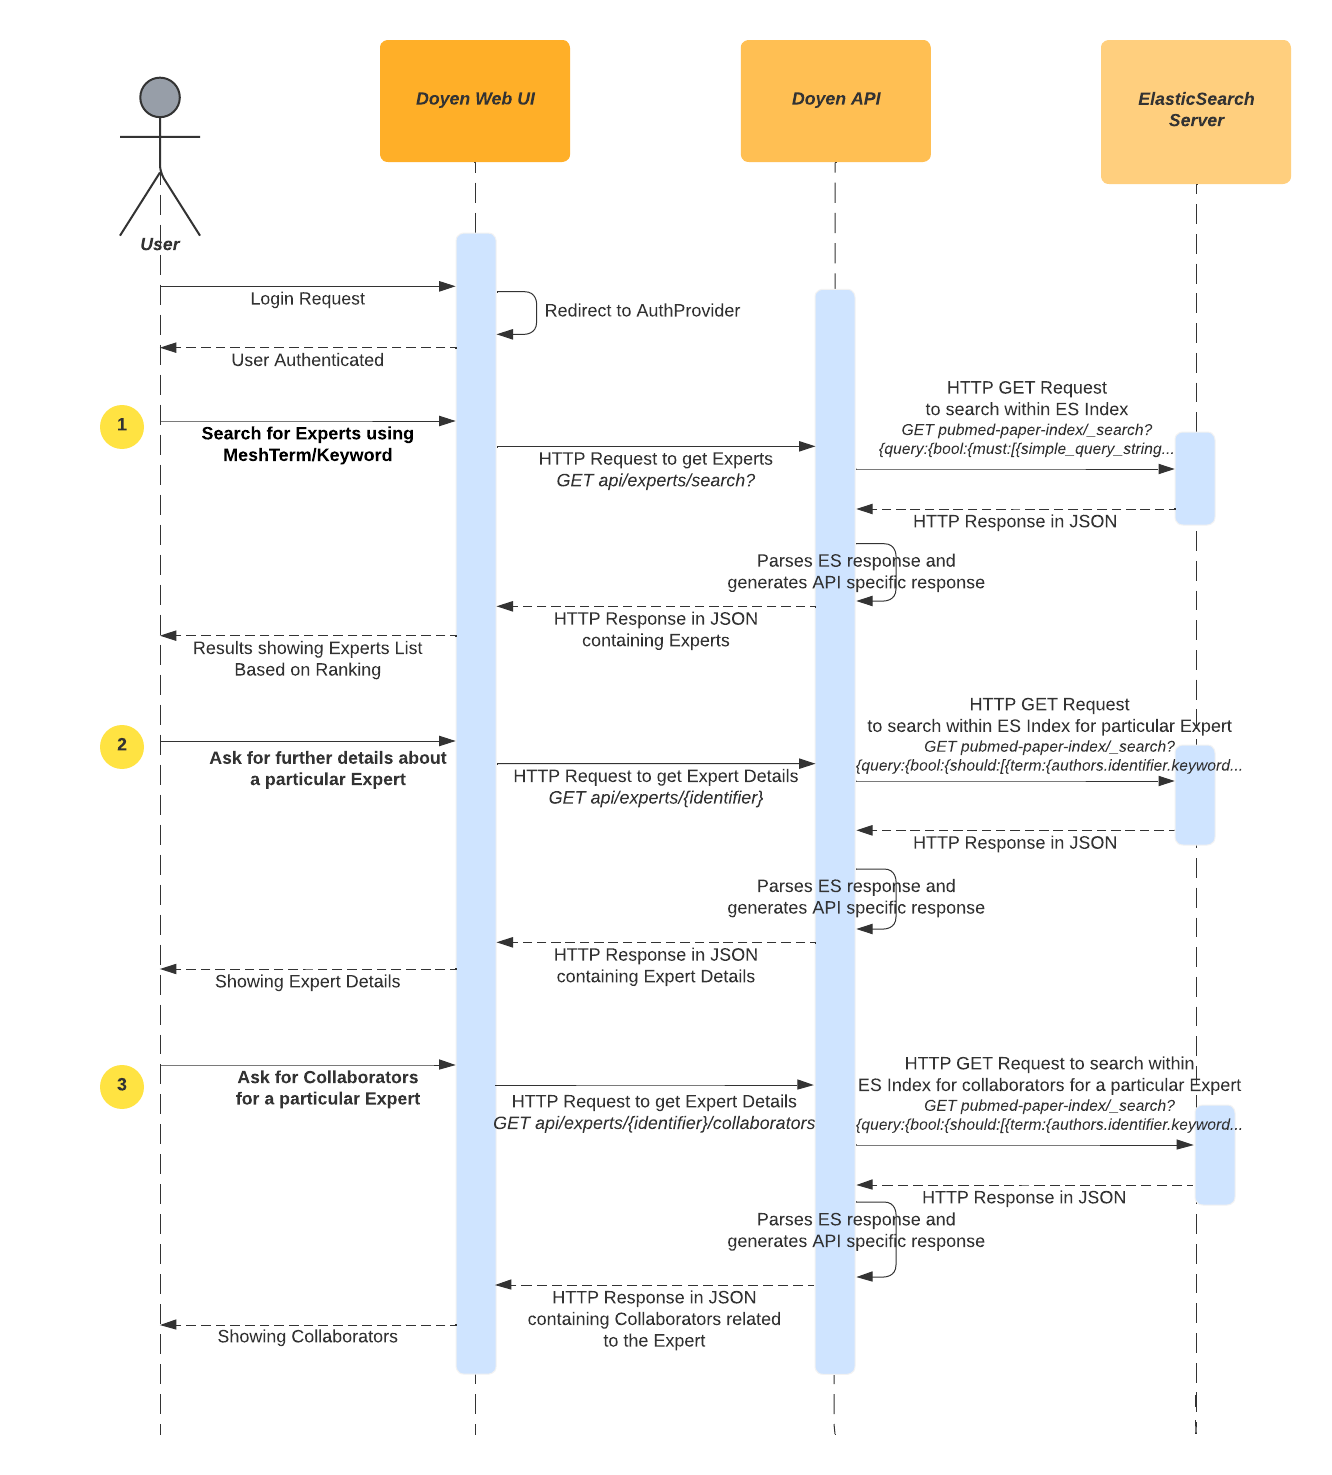
\includegraphics[width=\textwidth]{Images/SequenceDiagram_GetExperts.png}
    \caption{End-to-end flow - Sequence Diagram}
    \label{fig:sequence-diagram}
\end{figure}


\subsection{Front-End}

For the front-end of our application, we chose to implement the client using Next.js 13, a popular and efficient React framework for building user interfaces. Next.js allows us to create modular and reusable components, enhancing our application's development speed and maintainability.

In addition to Next.js, we utilized Tailwind CSS as our front-end styling framework. Tailwind is a highly customizable, low-level CSS framework that promotes a utility-first approach to styling. This choice enabled us to quickly build consistent, responsive, and performant user interfaces with minimal CSS overhead.

\subsection{Back-End}

Our back-end services are hosted on Amazon Web Services (AWS) EC2 instance and Azure. AWS EC2 allows users to launch Virtual Machines on the Amazon Cloud infrastructure with various workloads and application combinations. This choice allows us to focus on our application's functionality while AWS handles the scaling and maintenance of the underlying infrastructure. The API Gateway is the entry point for our back-end services, providing a fully managed service for creating, publishing, and maintaining secure APIs.

We implemented our data ingestion layer  using PySpark, a Python library for Apache Spark. PySpark allows us to process large-scale data in parallel, enabling efficient data manipulation and transformation. Furthermore, we built our ingestion pipeline using Python.

The back-end service API layer is implemented in .Net using C\# and hosted on Microsoft Azure Cloud. This combination enables us to build scalable and maintainable server-side applications while leveraging the vast ecosystem of Microsoft .Net libraries and tools.

\subsection{Ingestion Pipeline}

Our system has an ingestion pipeline workflow, shown in \autoref{fig:ingestion-flow}, which automatically downloads baseline data from the PubMed FTP server and processes it. The processed data is then stored in an Elasticsearch instance, which is hosted on an EC2 instance inside a Docker container. The ingestion pipeline is also located on the same EC2 instance and runs on demand.

To keep the Elasticsearch index up-to-date, we have implemented a daily cron job that downloads the daily update PubMed file from the Ftp server and runs the same ingestion pipeline. This ensures that the Elasticsearch index is always up-to-date and reflects the latest changes in the Pubmed database.

By automating the data ingestion process and implementing the daily cron job, we have reduced the manual effort required to update the Elasticsearch index, minimized the risk of errors and inconsistencies, and ensured that our system is always working with the most up-to-date data.

\begin{figure}[htp]
    \centering
    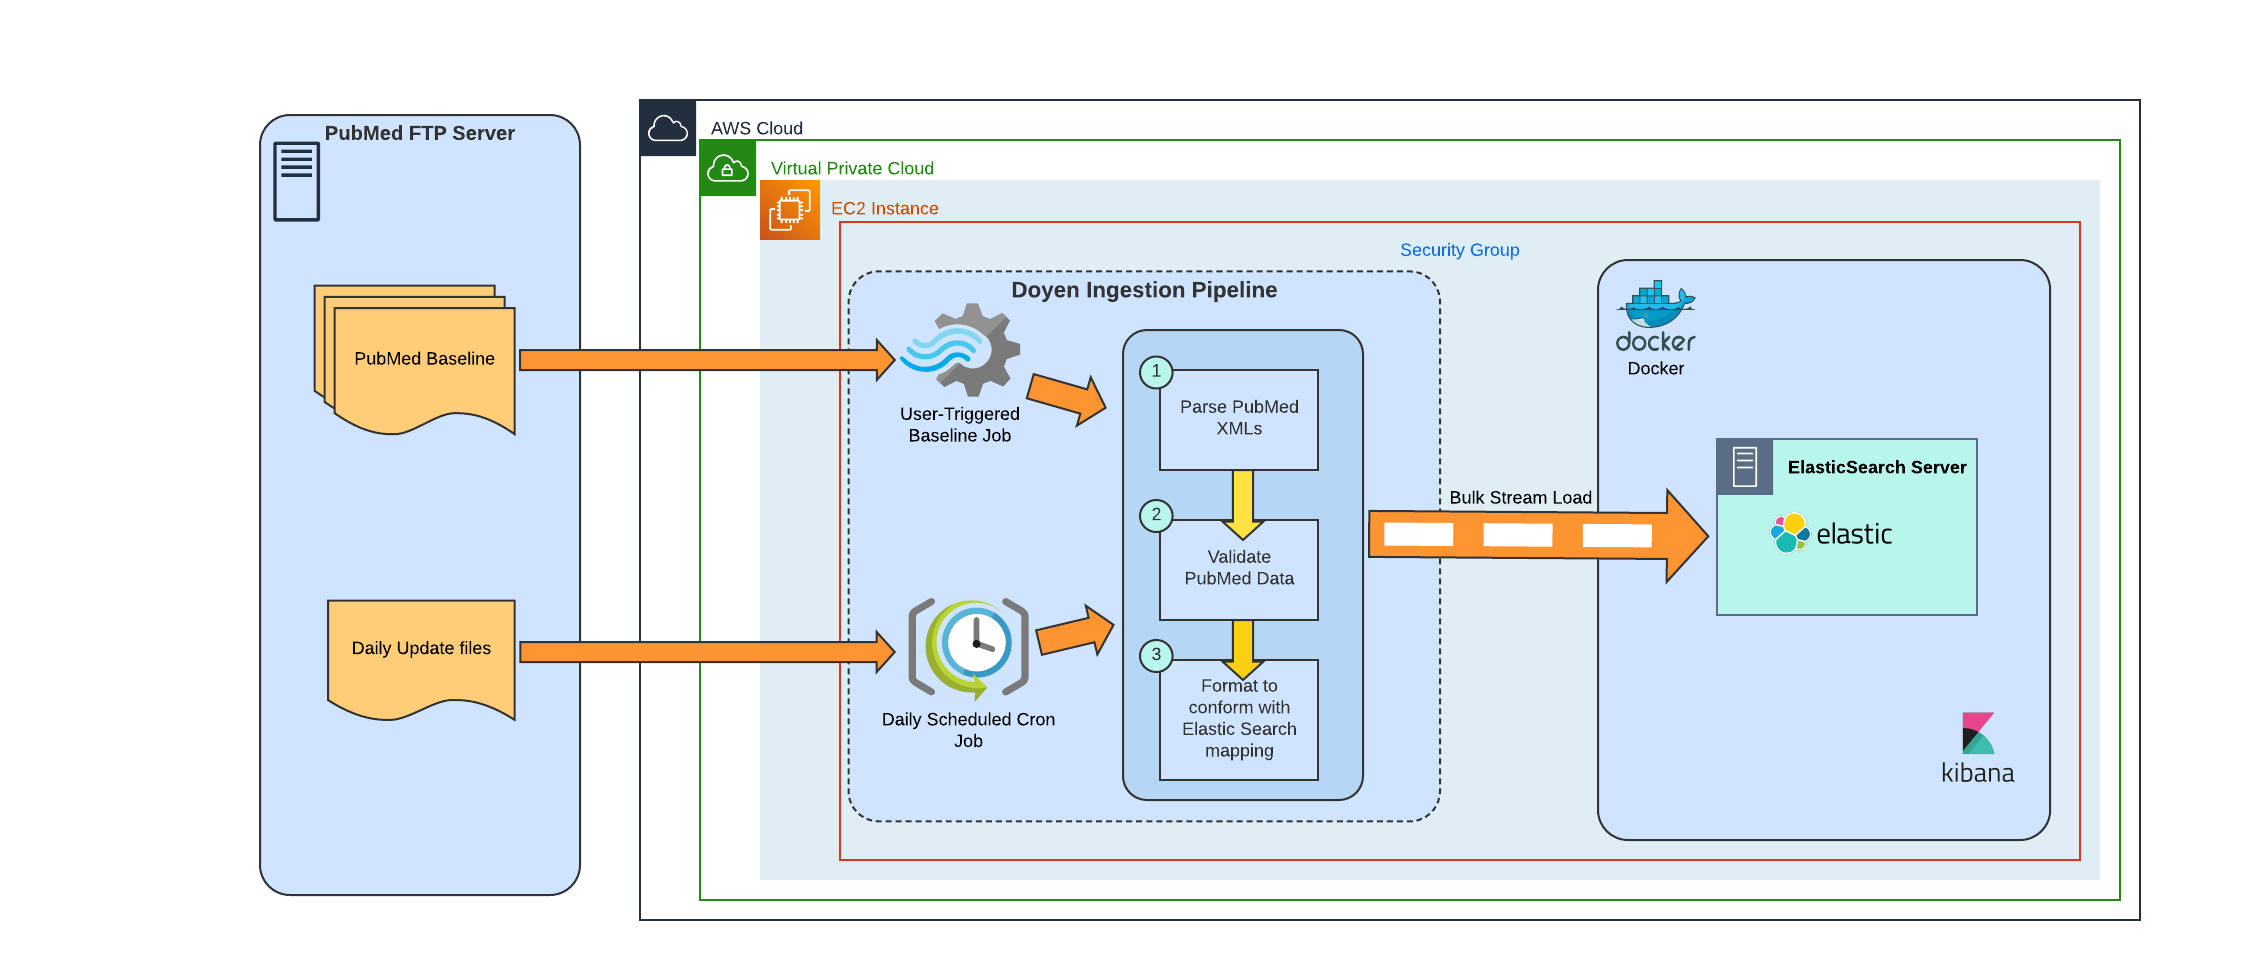
\includegraphics[width=\textwidth]{Images/Ingestion Pipeline flow.png}
    \caption{Ingestion Pipeline Flow}
    \label{fig:ingestion-flow}
\end{figure}


In \autoref{fig:ingestion}, you can see the Ingestion Pipeline comprises several classes, with the main entry point being the PubmedProcessor class. This class contains functions to create the Elasticsearch PubMed index and ingest files, utilizing the Elasticsearch and NihFtpClient libraries.

\begin{figure}[htp]
    \centering
    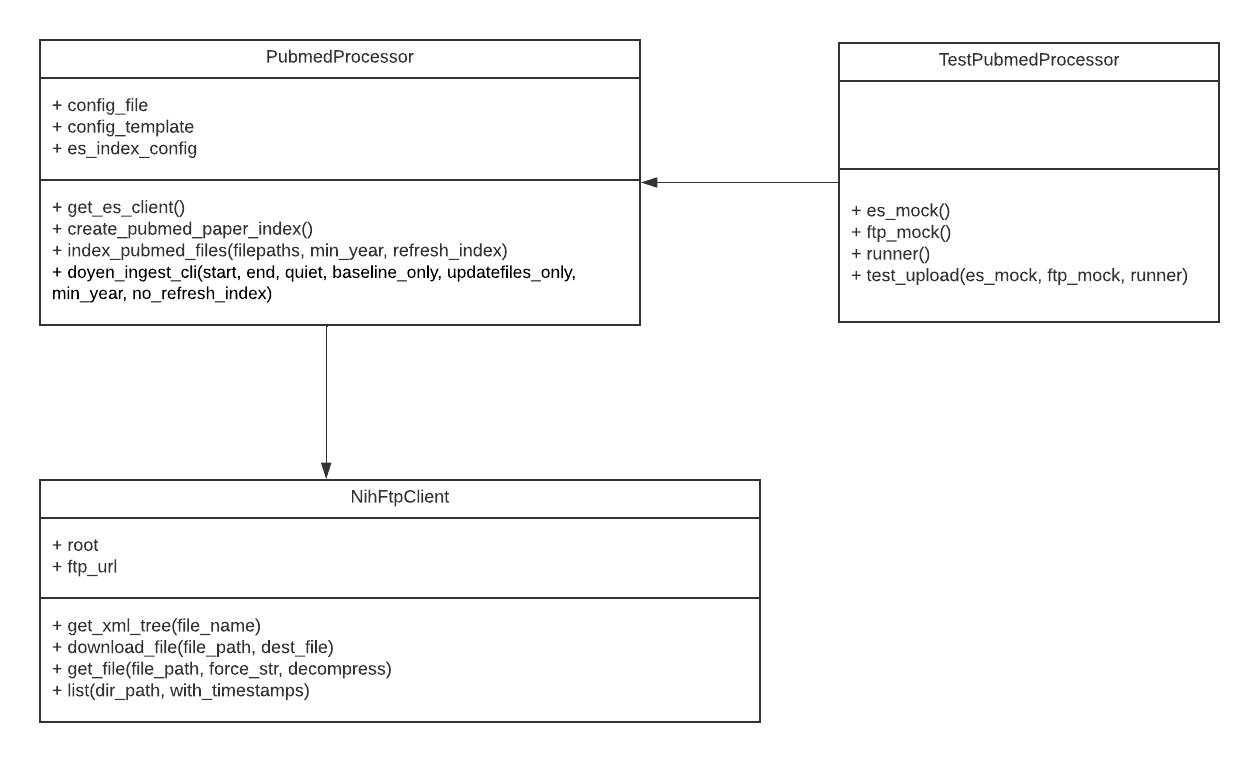
\includegraphics[width=\textwidth]{Images/IngestionPipeline_ClassDiagram.png}
    \caption{Ingestion Pipeline Model - Class Diagram}
    \label{fig:ingestion}
\end{figure}



\subsection{API Layer}

The API layer, shown in \autoref{fig:api-layer} is a crucial component that facilitates communication between the front-end and back-end. It serves as the primary interface for the front-end to interact with the back-end services. The API layer is responsible for managing and processing incoming requests from the front-end and sending them to the Elasticsearch Server for data retrieval. It executes queries against the server to retrieve the desired data and refines and translates it into a format that is easily digestible for the front-end.

Apart from basic search queries, the API layer is also responsible for running advanced queries, such as aggregated queries, to extract expert-related information like collaborators, research interests, and more. The API layer plays a vital role in providing a seamless user experience, ensuring that data is processed and delivered efficiently and accurately. It also allows the system to be extensible, bringing in additional or changing data sources to supplement current data  without breaking the interface to the UI.


\begin{figure}[htp]
    \centering
    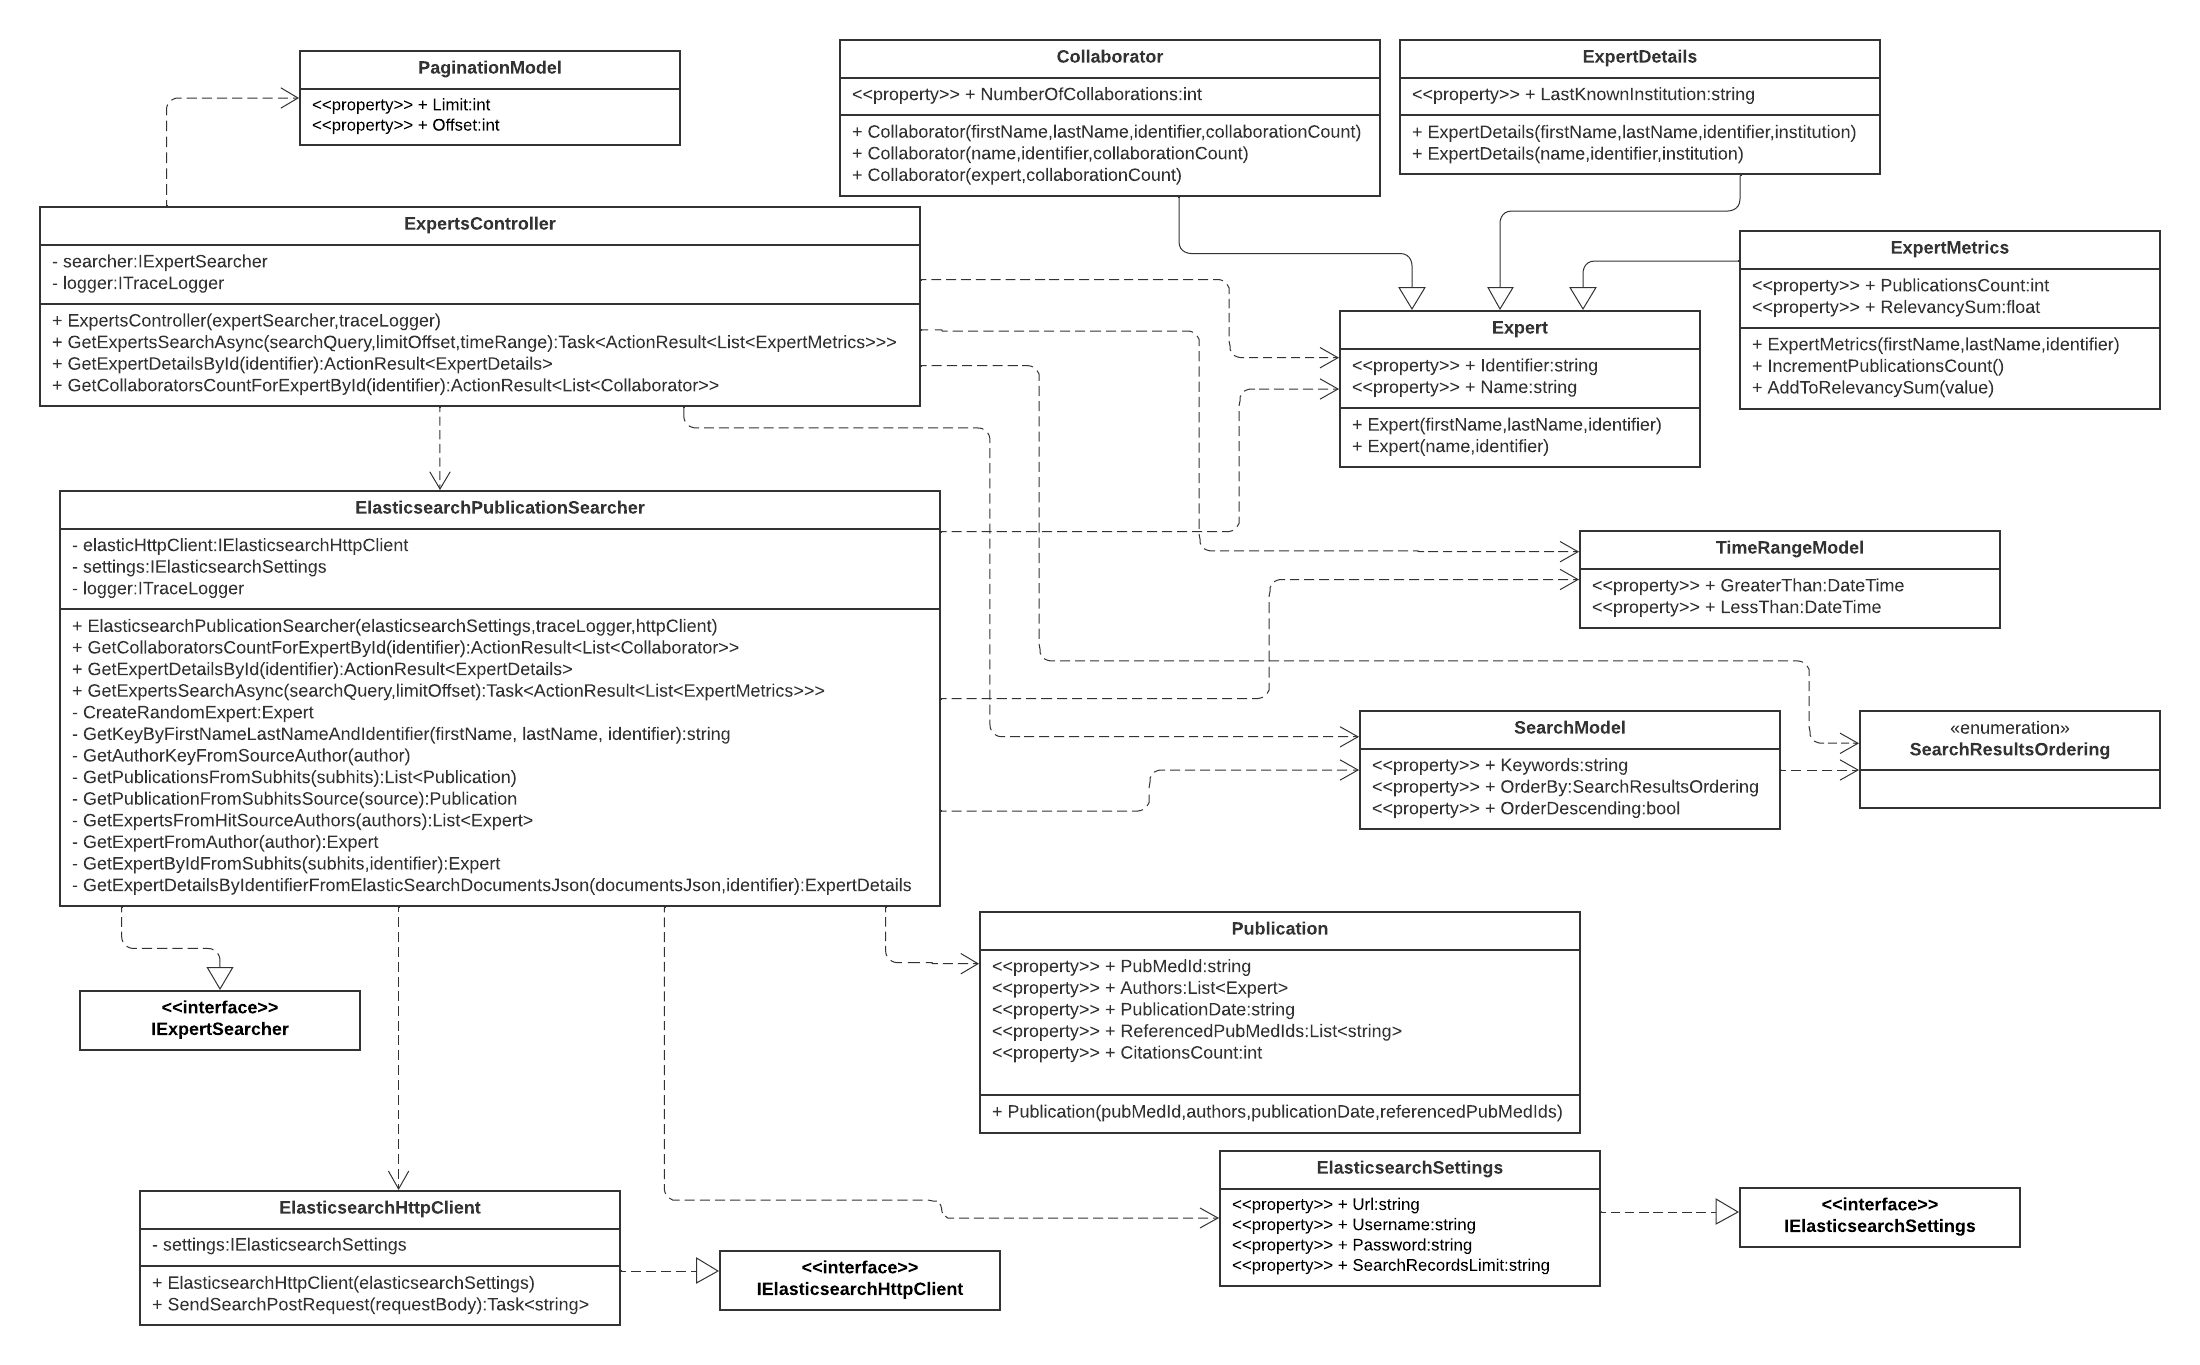
\includegraphics[width=\textwidth]{Images/API_ClassDiagram.png}
    \caption{API Layer - Class Diagram}
    \label{fig:api-layer}
\end{figure}

\subsection{Data Management}

Our primary data is hosted and searched using Elasticsearch, a powerful and flexible search and analytics engine. Elasticsearch allows us to store, search, and analyze large volumes of data quickly and in near real-time.

Additionally, we store extra data in Amazon Simple Storage Service (S3), a highly-scalable and durable object storage service. Amazon S3 provides a cost-effective, secure solution for storing and retrieving extensive data.

\subsection{Cloud Provider}

For our cloud provider, we selected Amazon Web Services (AWS). AWS offers a comprehensive suite of tools and services to help us build, deploy, and manage our application effectively and securely.

\subsection{Infrastructure}

As previously mentioned, our primary data is hosted in Elasticsearch. To manage our resource deployments, we utilized AWS CloudFormation,  enabling us to create and manage a collection of AWS resources using templates. This approach helped streamline infrastructure management and ensure a consistent and reproducible environment. The overall architecture is shown in \autoref{fig:architecture}.

We also use AWS CloudFront, a global content delivery network (CDN) service, to serve our front end. CloudFront accelerates the delivery of our application's assets by caching and distributing them across a network of edge locations, improving the overall user experience.
Our back-end is hosted on AWS Lambda and served through Amazon API Gateway, as discussed in section 2.2.

\begin{figure}[htp]
    \centering
    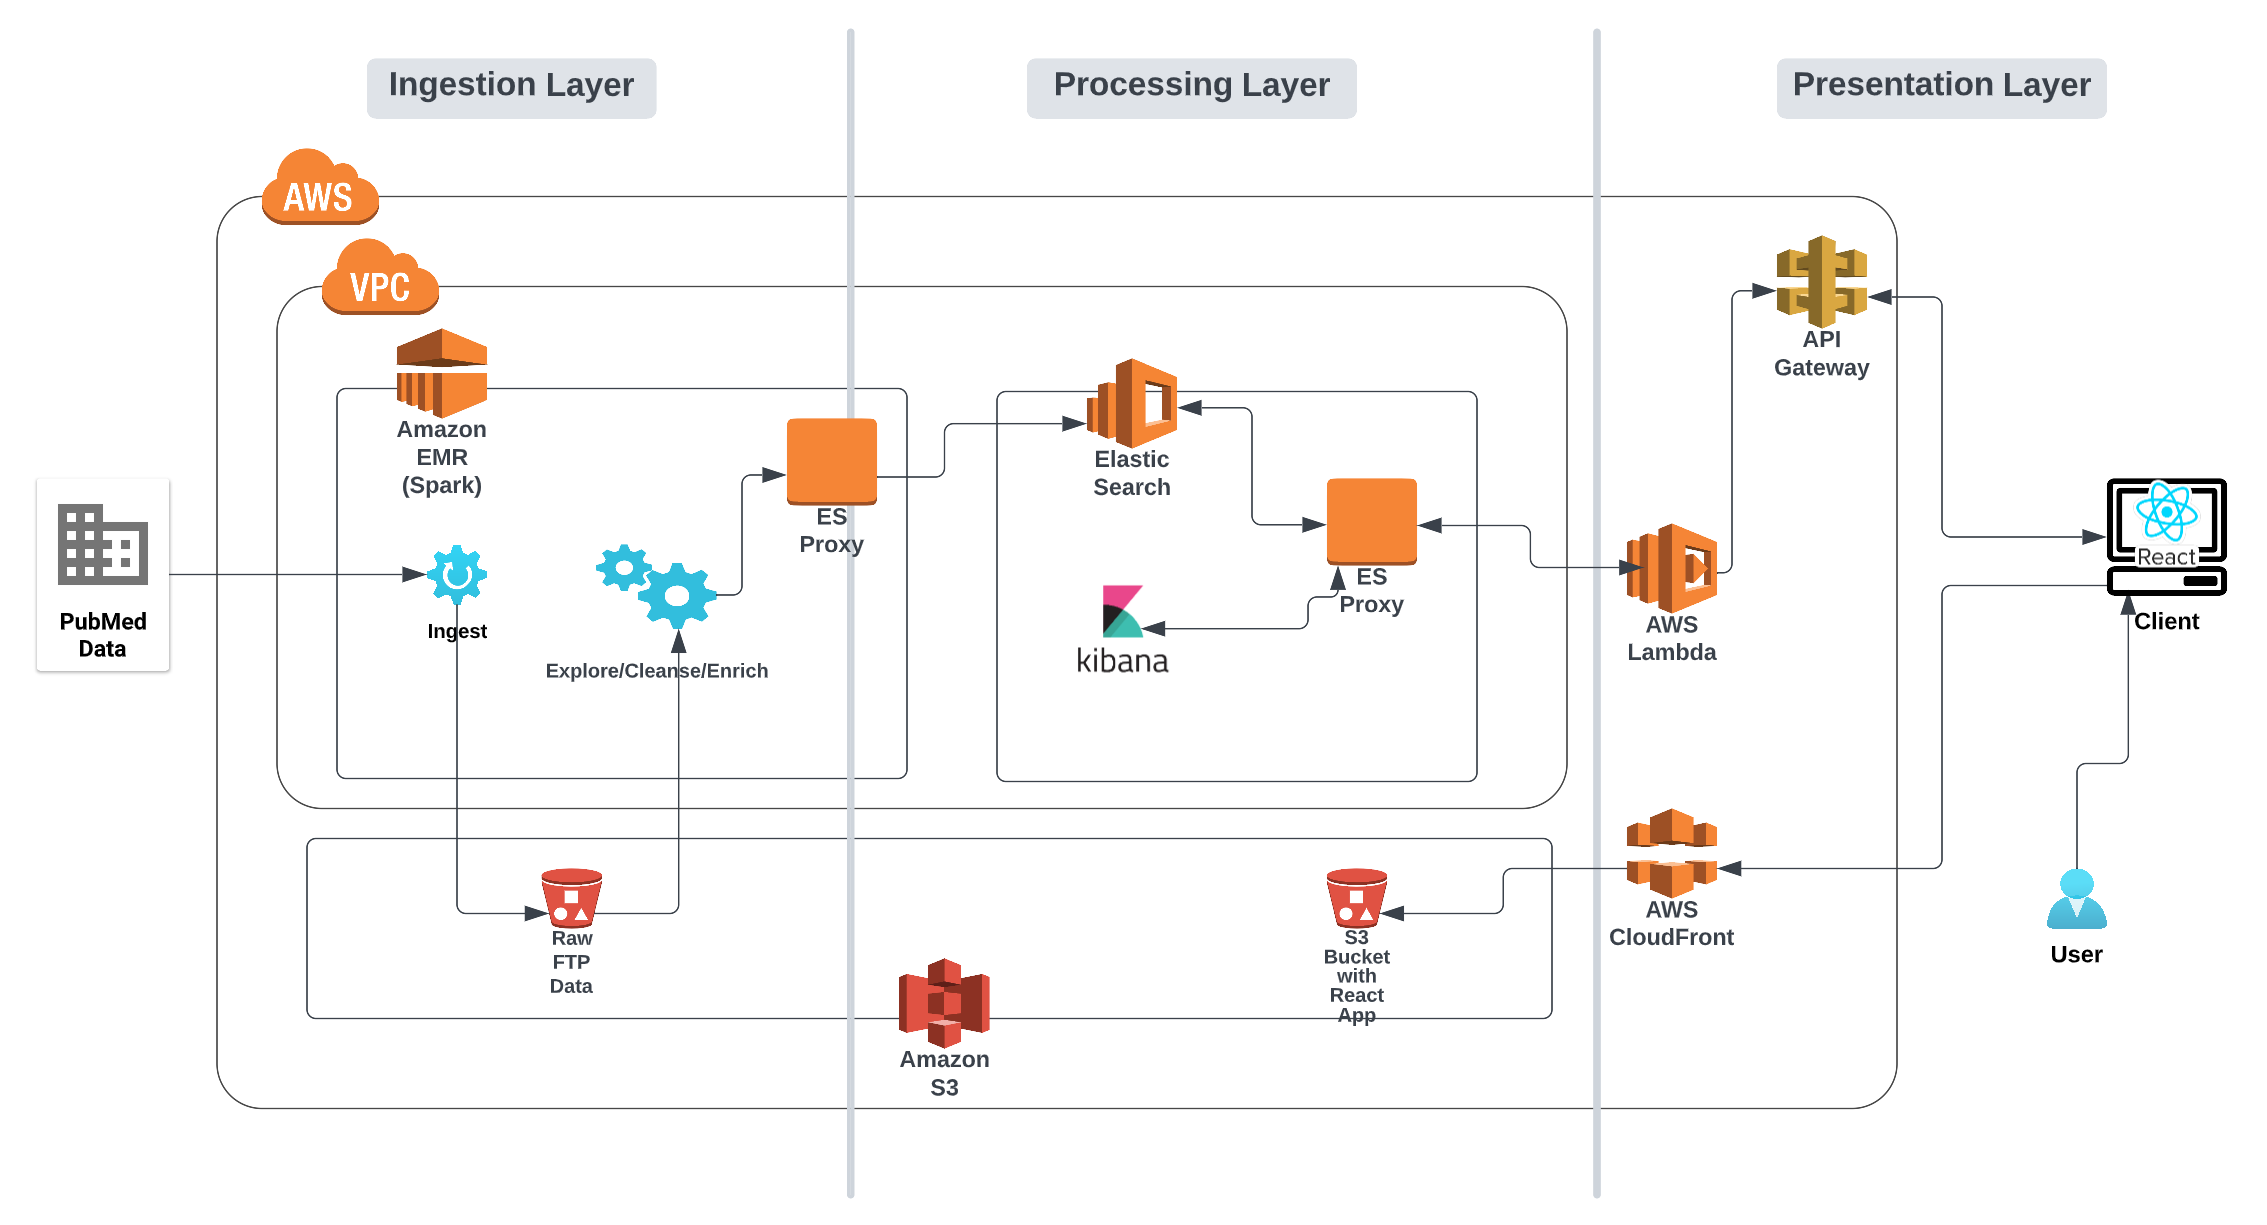
\includegraphics[width=\textwidth]{Images/Doyen High-Level Architecture Diagram.png}
    \caption{The Doyen Architecture}
    \label{fig:architecture}
\end{figure}

\subsection{Version Control and CI/CD}

We used GitHub for version control, allowing us to manage our codebase effectively, track changes, and collaborate efficiently. GitHub also implements our continuous integration/continuous delivery (CI/CD) pipeline. This pipeline automates the process of building, testing, and deploying our application, ensuring we maintain a high code quality and consistency throughout the project's lifecycle. By implementing a CI/CD pipeline, we can detect and address issues early, reduce manual intervention, and streamline the delivery of new features and bug fixes.

In conclusion, our project's design incorporates modern and scalable technologies to ensure a robust and maintainable application. Our choice of AWS as a cloud provider, combined with implementing CloudFormation, CloudFront, and a CI/CD pipeline using GitHub, allows us to streamline our infrastructure management and ensure a consistent and reproducible environment for our application. By utilizing Next.js, Tailwind CSS, Elasticsearch, AWS Lambda, and API Gateway, we built an efficient and responsive front-end and a reliable and scalable back-end and effectively manage our data.

\section{Testing}

During the course of our project, we conducted various types of testing to ensure the quality and functionality of our application. These tests included unit testing, manual testing by users and customers in the production environment, and more specialized tests for different aspects of the project.

\subsection{Ingestion Performance Tests}

We developed a test infrastructure for the back-end pipeline, focusing on the performance of data ingestion. While we recognized the need to handle large amounts of data in the pipeline, we faced the challenge of mocking this data and incorporating it into our tests. Due to these constraints, we prioritized other aspects of the project and implemented only limited tests for the ingestion performance.

\subsection{User Acceptance Tests}

We collaborated closely with the client throughout the project to meet their requirements and gather valuable feedback. By demonstrating our progress at various stages, we obtained actionable insights that allowed us to refine and enhance the project. This iterative approach ensured that our application met the needs and expectations of its users.

\subsection{UI Tests}

To maintain the quality and functionality of the user interface, we conducted both unit and integration tests for the various components. We utilized Cypress, a JavaScript-based tool using DOM manipulation for automated web tests, to simulate user interactions and assess the performance of our UI components. Currently, we have approximately 30 tests covering essential front-end features such as site navigation, query results, and interactive table functionalities like sorting and filtering. The Cypress testing dashboard can be seen in \autoref{fig:ui-tests}.

\begin{figure}[htp]
    \centering
    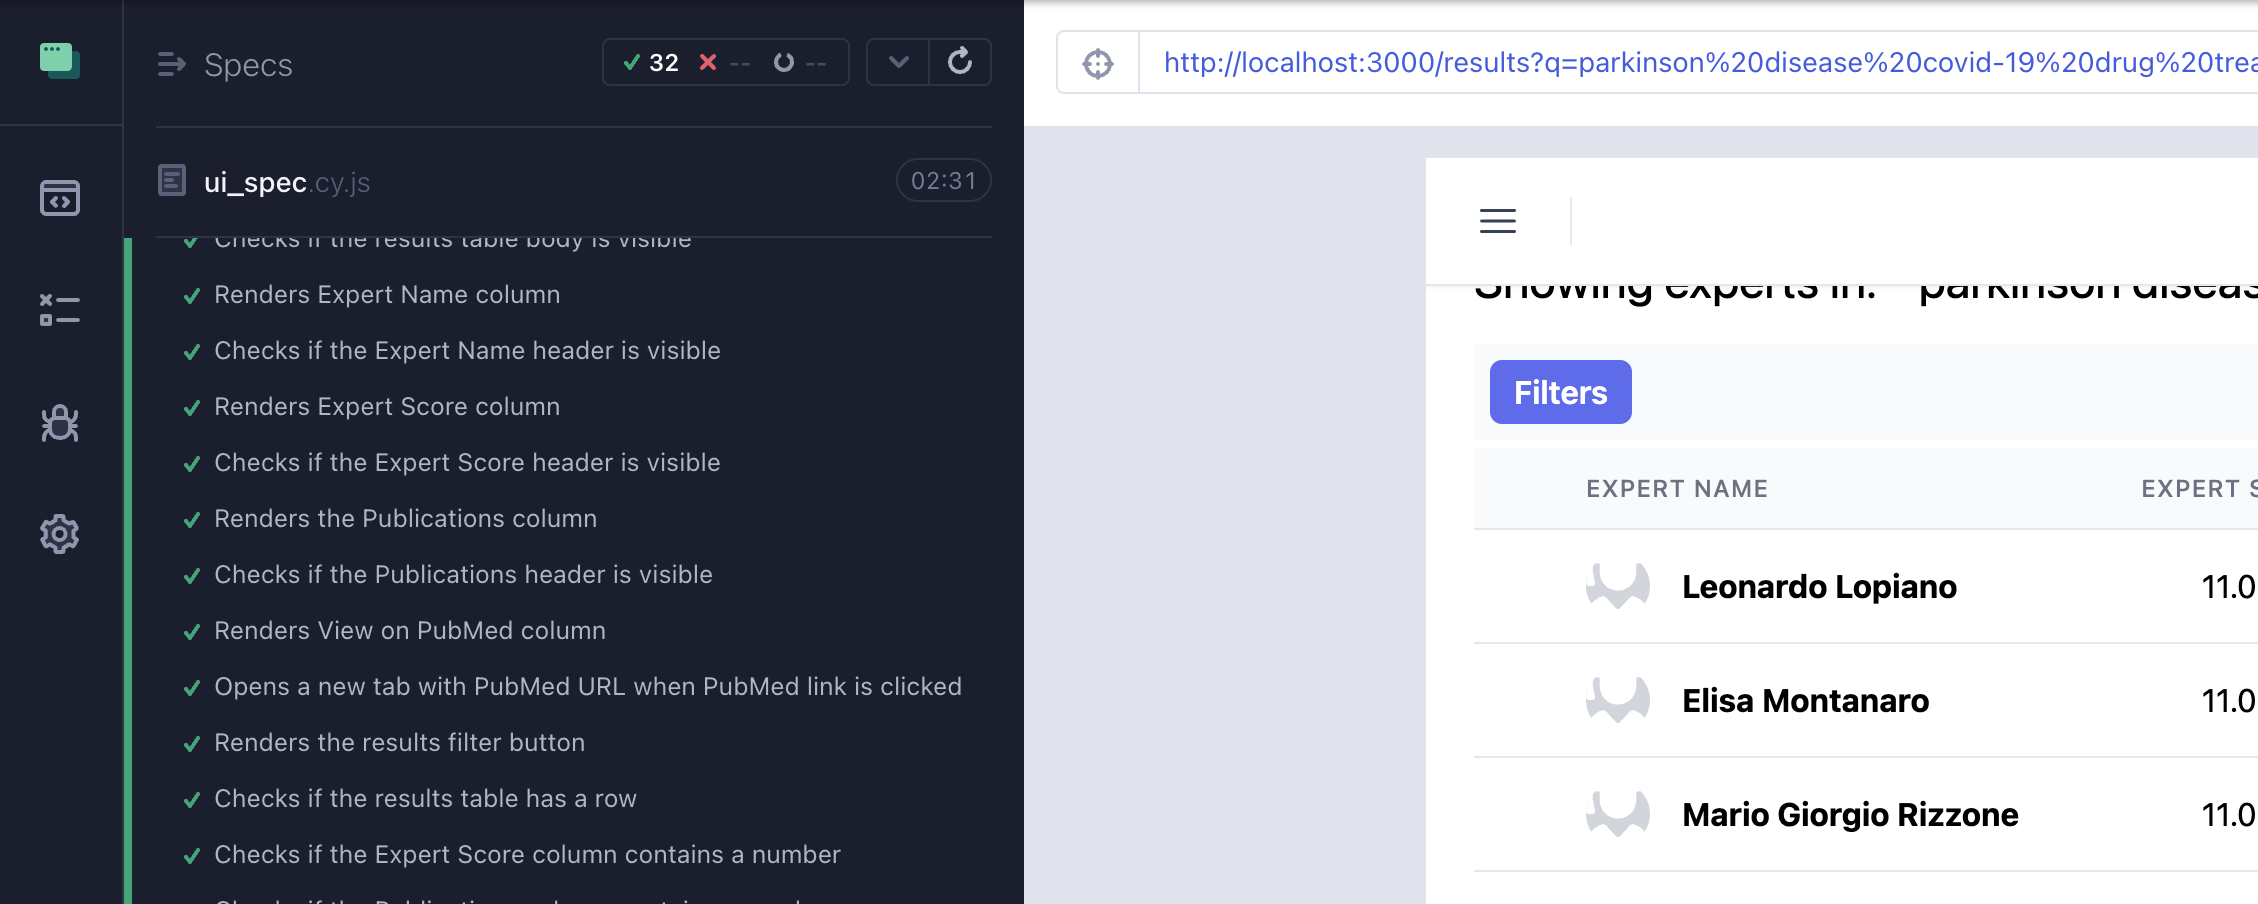
\includegraphics[width=\textwidth]{Images/ui-tests.png}
    \caption[UI Test Results in Cypress Dashboard]{\textbf{A view of the Cypress dashboard showing UI test results:} The Cypress dashboard displays the UI spec testing file, showing 32 passing tests related to user interface functionality. }
    \label{fig:ui-tests}
\end{figure}

\subsection{API Tests}

We employed Postman for API testing in order to validate the requests and responses of our Next.js app's API endpoints. Postman's Runner feature allowed us to simulate front-end application behavior by executing a series of requests concurrently. Currently, we have three endpoints being tested with approximately 20 separate tests in the production environment, all passing successfully, as seen in \autoref{fig:api-tests}.

\begin{figure}[htp!]
    \centering
    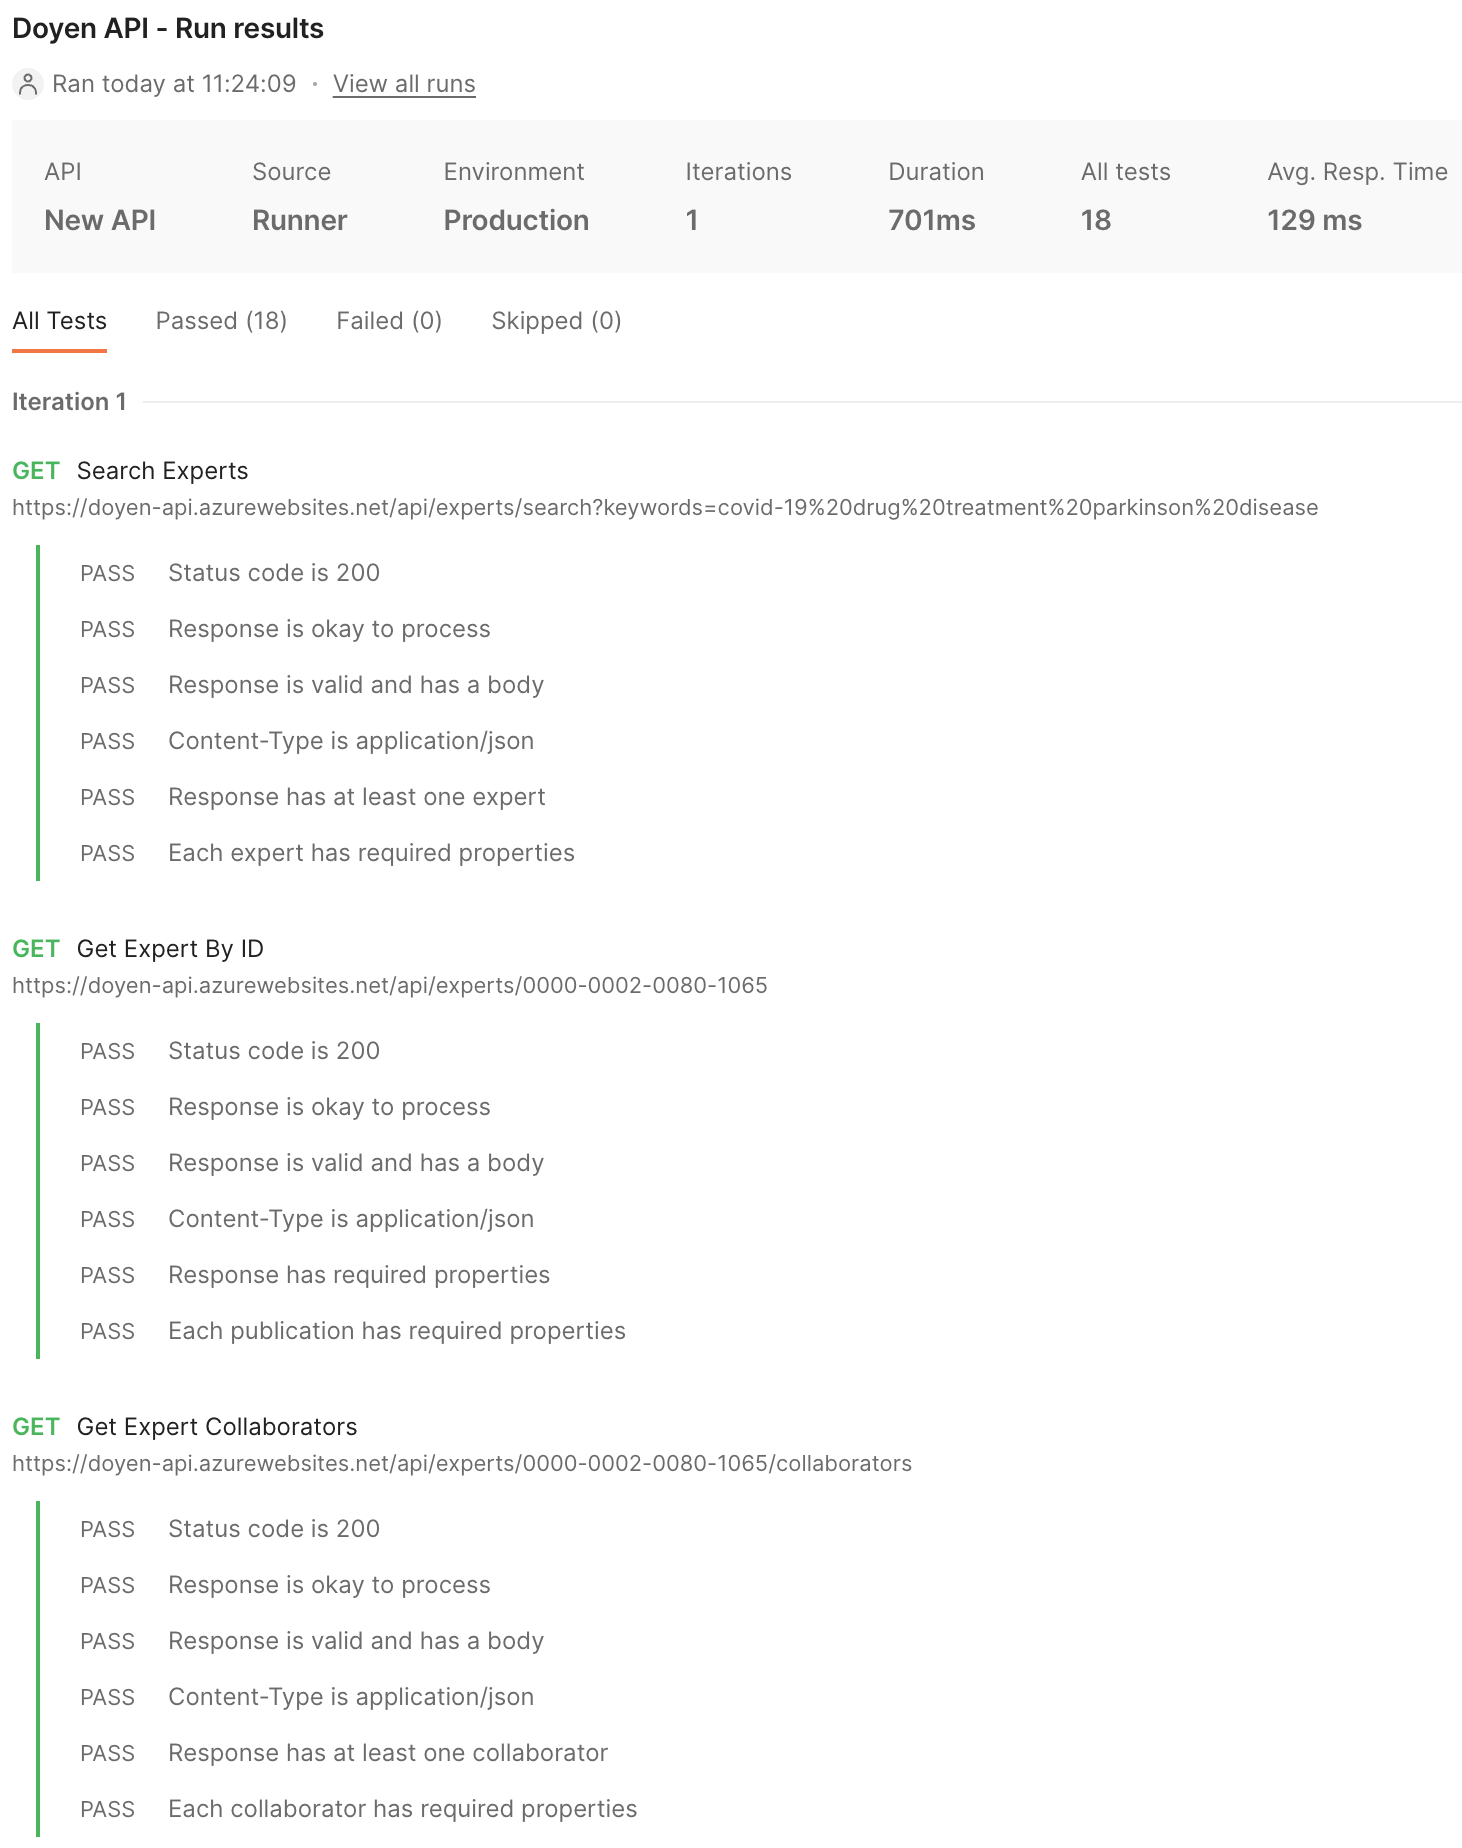
\includegraphics[width=\textwidth]{Images/api-tests.png}
    \caption[API Test Results in Postman Dashboard]{\textbf{A view of the Postman dashboard showing API test results:} The Postman dashboard displays the Doyen API run results, showing 18 passing tests across the three Doyen API endpoints. }
    \label{fig:api-tests}
\end{figure}

In conclusion, by incorporating these various testing methods, we sought to ensure the robustness and reliability of our application while continuously refining its features based on user feedback and requirements. The testing process played a crucial role in the overall success of our project, helping us identify and address potential issues before they could negatively impact the end-user experience.

\section{Tool Suite}

Here we describe the tools we as a team will use in executing this project.

\subsection{Communication}
We used online text and chat tools for our primary means of communication:
\begin{itemize}
    \item Discord: Used for day-to-day communication between team members. We have three channels:
    \begin{itemize}
        \item General: we discuss upcoming deadlines, ask questions still unanswered from meetings, and discuss possible alternatives to current work.
        \item Daily stand-up: Each member posts a daily update of what they have done the previous day, what they are doing today, and any blockers present. 
        \item Research papers: A channel that houses all of the research that we have found related to any part of the project. 
    \end{itemize}
    Discord also allows any-time voice or video calls through the voice channel.
    \item Email: Used to communicate with the client.
\end{itemize}

\subsection{Version Control and CI/CD}
We used git and GitHub for all of our version control, and we used GitHub actions for CI/CD. We used a team repository where pull requests inform the team members of any desired changes to the codebase. This houses front-end code, server code, and any microservices. Upon each accepted commit to the production branch, a continuous integration and delivery pipeline runs the build and appropriate tests using GitHub Actions.

\subsection{Backlog}

We used GitHub issues to track backlog tasks and issues.

\subsection{File Sharing}

We used cloud tools for sharing files
\begin{itemize}
    \item Google Drive: Used this to share working files, e.g. meeting notes. 
    \item Overleaf: We used this for working on our core research paper document and the milestones we create from that.
\end{itemize}

\subsection{Documentation}
We used Swagger for our API documentation and published further documentation through GitHub pages, with possible integrations of various auto-doc generators for the different layers of our application to document the code.


\vfill
\pagebreak

%%%%%%%%%%%%%%%%%%%%%%%%%%%%%%%%%%%%%%%%%%%
% Appendices
%%%%%%%%%%%%%%%%%%%%%%%%%%%%%%%%%%%%%%%%%%%

\begin{appendices}

\section{Team Strategy and Dynamics}

We organized to tackle the project by discussing team members’ backgrounds and surveying them to gauge the skill set of each team member. The plan is to get contributions from every team member and keep the balance between learning and utilizing the existing skill set. This balance will be maintained through feedback and discussion.

We will be largely following an agile strategy for organizing our work and will make decisions by a consensus process if disagreements come up. We have set up a discord server to discuss project-related issues and get instant feedback from the team members. We have internal meetings twice a week and customer meetings once per week. We will meet each week, on Monday evenings and:
\begin{enumerate}
    \item Sprint Review
    \item Retrospective
    \item Review the Backlog
    \item Plan the next Sprint
\end{enumerate}
We will also have a standing meeting with the customer once weekly on Fridays and can meet more or less as needed. In summary:
\begin{itemize}
    \item Sprints - Weekly
    \item Roles - Flat structure, with specialization into aspects of the project as needed.
    \item Ceremonies - Daily standup (on Discord)
    \item Backlog refinement - Part of our weekly meetings
    \item Sprint Planning - Part of our weekly meetings
    \item Daily Scrum - Daily standup (on Discord)
    \item Sprint Review - Part of our weekly meetings
    \item Retrospectives - Part of our weekly meetings
\end{itemize}


\section{Doyen Team Contract}

\begin{itemize}
    \item We will communicate primarily through Discord when not in person.
    \item We will meet on Mondays at 7:30pm ET, and otherwise as arranged as needed.
    \item Time zones:
    \begin{itemize}
        \item Nicholas - PST
        \item Edwin - EST
        \item Patrick - EST
        \item Jeremiah - PST
        \item Muhammad - EST
    \end{itemize}
    \item Before the team meeting, team members should:
    \begin{itemize}
        \item Contribute to the shared agenda
        \item Have questions, comments, or ideas related to the agenda
    \end{itemize}
    \item We will structure our work as follows:
    \begin{itemize}
        \item We will work asynchronously via GitHub and its projects/issues.
        \item We will break the work into week-long sprints with a customer demo each week.
        \item We will have a daily stand-up in Discord text, which answers the following questions:
        \begin{itemize}
            \item What did you do yesterday?
            \item What will you do today?
            \item Are there any impediments in your way?
        \end{itemize}
    \end{itemize}
    \item We will submit assignments as follows:
    \begin{itemize}
        \item The team works independently for individual submissions.
        \item The team will agree upon a due date for collaborative submission for each member to complete their portions before submission.
    \end{itemize}
    \item Surprises will be handled as follows:
    \begin{itemize}
        \item Daily stand-ups via Discord will inform the team as early as possible.
        \item The team will try not to build silos. We can try to overlap skills within the project’s subsystems.
    \end{itemize}
    \item Turn-taking will be managed as follows:
    \begin{itemize}
        \item We’ll make space at the end (and often the beginning) of each to give each team member space to speak and share their thoughts.
    \end{itemize}
    \item Conflict will be handled as follows:
    \begin{itemize}
        \item If it is a disagreement on our method, we will use a consensus process to try to resolve the disagreement.
        \item Speak with each other.
        \item Speak openly about struggles.
        \item Speak with TF as a neutral third party for a final fallback.
        \item Don’t take other people’s work without consent (within reason – someone could be very, very far behind).
    \end{itemize}
    \item Other considerations:
    \begin{itemize}
        \item Brainstorming / Design Critiques:
        \begin{itemize}
            \item Use building language and constructive criticism.
            \item Compliment sandwiches when needed.
        \end{itemize}
    \end{itemize}
\end{itemize}


\end{appendices}



\end{document}